\section{Main Objectives}


\begin{frame}
\frametitle{}
	\framesubtitle{}

\begin{textblock*}{250pt}(120pt,130pt)
\Huge
\textbf{Graduate Seminar 2}
\end{textblock*}

\end{frame}





\begin{frame}
\frametitle{Quantum theory of radiation by nonstationary systems 
	with application to high-order harmonic generation
        (Phys. Rev. A 101, 013410 (2020))}
        \framesubtitle{Part 1 - Solving $\boldsymbol{\psi(x,t)}$}
\footnotesize
\begin{textblock*}{400pt}(30pt,60pt)
\begin{itemize}
\item To this end, we need to resolve $\psi(x,t)$ 
which is given by the regular TDSE, i.e 
\begin{equation}
	i\frac{\partial}{\partial t}\psi(x,t)
	   = \left( \hat{H}_a + \hat{V}_{\rm ext}(t)\right) 
	   \psi(x,t),   \hspace{20pt}\psi(x,0)=\psi_0(x),  \label{eqn:step_1d}
\end{equation}
\begin{equation}
  \hat{H}_a = -\frac{1}{2}\frac{d^2}{dx^2} - \varkappa\delta(x), \hspace{20pt}
  \hat{V}_{\rm ext} = F(t)x,
\end{equation}
\begin{equation}
  E_0 = -\varkappa^2/2,\hspace{20pt}
  \psi_{0}(x) = \varkappa^{1/2}e^{-\varkappa|x|}, \hspace{20pt}
  \varkappa = 1       \label{eqn:bound_state}
\end{equation}
\begin{equation}
  E_k = k^2/2,\hspace{20pt}
  \psi_k^{(\pm)}(x) = e^{ikx} + R(\pm|k|)e^{\pm i|kx|}, \hspace{20pt}
   R(k) = \frac{i\varkappa}{k-i \varkappa}. \label{eqn:inout_states}
\end{equation}
\vspace{10pt}
\item The parameters of the laser we will be using 
are given by the relations
\begin{equation}
  F(t) = F_0 e^{-(2t^\prime/\tau)^2}\cos(\omega_0 t^\prime),
\hspace{20pt}  0 \leqslant t \leqslant T,
\hspace{20pt}  t^{\prime} = t - T/2,
\end{equation}
\begin{equation}
  \tau  = 2\pi n_{oc}/\omega_0,  \hspace{20pt}
  n_{oc} = 5. \hspace{20pt}
\end{equation}
\end{itemize}

\end{textblock*}

\begin{textblock*}{250pt}(240pt,80pt)
%\includegraphics[scale=.25]{dip_app_limits.png}{\footnote{\Tiny
%H.R. Reiss, Phys Rev A 63 013409 (2000)}}
\end{textblock*}

\end{frame}




\begin{frame}
\frametitle{Quantum theory of radiation by nonstationary systems 
	with application to high-order harmonic generation
        (Phys. Rev. A 101, 013410 (2020))}
	\framesubtitle{Survival probability and PEMD}

\begin{textblock*}{400pt}(30pt,60pt)
\footnotesize
\begin{itemize}
\item The coefficients of the projection of $\bar{\Psi}$ are then, at $T$,
and by definition, expressed as
\begin{equation}
a_0 = e^{iE_0 T}\int \psi_0(x) \psi(x,T)dx, \hspace{20pt}
a_k = e^{iE_k T}\int \psi_k^{\Tiny (-)*}(x) \psi(x,T)dx. \hspace{20pt}
\label{eqn:a0k}
\end{equation}

%with 
%$\bar{\Psi}_{k_j} = a_{k_j} 
%\hspace{10pt} 0\leqslant j \leqslant m$, \hspace{30pt}
%$\bar{\Psi} = \left( \bar{\Psi}_0, \bar{\Psi}_{k_1}, \cdots, \bar{\Psi}_{k_j}
%\cdots, {\Psi}_{k_m}\right)$.


\item The survival probability is then expressed, 
at the end of the interaction, by
\begin{align}
   P_0         & = \left| a_0 \right|^2. \label{eqn:surv}  
\end{align}

\item The ionization probability can then be found many different 
ways that should be consistent with each others
\begin{align}
   P_{\rm ion} & = \int P(k)\frac{dk}{2\pi}, 
 \hspace{30pt} \mbox{with}\hspace{30pt} P(k) = \left| a_k \right|^2. 
\label{eqn:pion1} \\
               & = 1-P_0.
\end{align}

\item  $P(k)$ is the probability for the electron 
being ionized with the energy $E_k$.

\end{itemize}
\end{textblock*}


\end{frame}



\begin{frame}
\frametitle{Quantum theory of radiation by nonstationary systems 
	with application to high-order harmonic generation
        (Phys. Rev. A 101, 013410 (2020))}
	\framesubtitle{Quantum spectrum of HHG photons (semi-classical approx.) - 1}

\begin{textblock*}{400pt}(30pt,60pt)
\footnotesize
\begin{itemize}
\item In the classical approx., the spectrum is obtained from the following 
(Eq.(80))
\begin{equation}
Q^{(c)}_\nu (\omega) = 
 \alpha^2 \omega^2
    \left| \boldsymbol{\rm A}_{\nu}\boldsymbol{\rm d}(\omega) \right|^2,
\label{eqn:Qc}
\end{equation}
where for an arbitrary operator $\hat{f}$, we have   
\begin{equation}
f(t) = \int \psi^{*}(x,t)\hat{f}\,\psi(x,t)dx
\label{eqn:mean_value}
\end{equation}
and the Fourier transform is obtained using 
\begin{equation}
f(\omega) = \int f(t)e^{i\omega t}dt.
\label{eqn:fourier}
\end{equation}

\item Also, we consider the relations
\begin{align}
% \boldsymbol{\rm A}_\nu 
%   = \sqrt{\frac{2\pi c^2}{\omega L^3}}\boldsymbol{\rm e}_\nu,
%   \hspace{20pt}\alpha = 1/c.
 \hat{p} = -i d/dx, \hspace{20pt} \hat{d} = -x
\end{align}
\end{itemize}
\end{textblock*}


\end{frame}






\begin{frame}
\frametitle{Quantum theory of radiation by nonstationary systems 
	with application to high-order harmonic generation
        (Phys. Rev. A 101, 013410 (2020))}
	\framesubtitle{Quantum spectrum of HHG photons (semi-classical approx.) - 2}

\begin{textblock*}{400pt}(30pt,60pt)
\footnotesize
\begin{itemize}
\item Let us apply the following simplifications
\begin{align}
    \nu \longrightarrow \omega, \hspace{20pt}
  \boldsymbol{\rm A}_\nu = \sqrt{\frac{2\pi c^2}{\omega L^3}}\boldsymbol{e}_\nu
\longrightarrow A_\omega, 
    \hspace{20pt}\mbox{ and } \hspace{20pt} \alpha A_\omega = 1.
\end{align}
\item So the observable we are considering here is 
\begin{align}
    Q^{(c)}(\omega) = \omega^2 \left| d(\omega)  \right|^2.
\end{align}
\item Additionally let us consider Eq. (104)
\begin{align}
    Q^{(c)}(\omega) = \left| p(\omega)  \right|^2.
\end{align}
and, by virtue of $\boldsymbol{p}(t)= -\dot{\boldsymbol{d}}(t)$, which reads
\begin{align}
    Q^{(c)}(\omega) = \left| -\dot{d}(\omega)  \right|^2. 
\label{eqn:dipole_mom_diff}
\end{align}

\end{itemize}
\end{textblock*}


\end{frame}


\begin{frame}
\frametitle{Quantum theory of radiation by nonstationary systems 
	with application to high-order harmonic generation
        (Phys. Rev. A 101, 013410 (2020))}
	\framesubtitle{Length, velocity and acceleration gauges}

\begin{textblock*}{400pt}(30pt,60pt)
\footnotesize
\begin{itemize}
\item (\ref{eqn:mean_value}) applied to the operator $\hat{d}$ gives
its expression in the length gauge
\begin{equation}
d(t) = \langle \hat{d\,} \rangle = - \left\langle\hat{x}\right\rangle
  = - \int \psi^{*}(x,t)\hat{x}\,\psi(x,t)dx
\end{equation}

\item $\dot{d}(t)$ is given by the formula
\begin{equation}
\dot{d}(t) = \frac{d}{dt}d(t)
\end{equation}

\item $p(t)$ is given by the formula
\begin{equation}
p(t) = \langle \hat{p\,} \rangle  
  = - i\int \psi^{*}(x,t)\frac{\partial}{\partial x}\psi(x,t)dx
\end{equation}

\item Using the Ehrenfest theorem for the operator $x$, we get the relations 
\begin{align}
\frac{d}{dt}\langle \hat{x\,} \rangle 
        & = \frac{\langle \hat{p\,} \rangle}{m}, \\
\frac{d}{dt} \langle \hat{p\,}\rangle 
        & = \left\langle -\frac{\partial V_{\rm ext}}{\partial x} \right\rangle
\end{align}

and some others (see Bransden and Joachain p.531-532) 



\end{itemize}
\end{textblock*}


\end{frame}




\begin{frame}
\frametitle{Quantum theory of radiation by nonstationary systems 
	with application to high-order harmonic generation
        (Phys. Rev. A 101, 013410 (2020))}
	\framesubtitle{Additional formula from Ehrenfest theorem}

\begin{textblock*}{400pt}(30pt,60pt)
\footnotesize
\begin{itemize}
\item  Using the integration by parts formula, we get
\begin{equation}
   p(\omega) = \int_{-T/2}^{T/2} e^{i\omega t} \frac{dx(t)}{dt}dt,\hspace{30pt}
   u(t) = x(t),\;\;\; v(t) = e^{i\omega t},
\end{equation}
\noindent thus
\begin{align}
   p(\omega) & = \int_{-T/2}^{T/2} \frac{d}{dt}\Big(e^{i\omega t}x(t)\Big)dt
    -i\omega \int_{-T/2}^{T/2} e^{i\omega t}x(t)dt, \\
             & = \Bigg[ e^{i\omega t} x(t)\Bigg]_{-T/2}^{T/2}
               -i\omega \int_{-T/2}^{T/2} e^{i\omega t}x(t)dt. 
\label{eqn:additional}
\end{align}

So, we get an additional formula for evaluating 
\begin{equation}
Q^{(c)}(\omega) = \left| p(\omega) \right|^2,
\end{equation}

\noindent with $p(\omega)$ evaluated conformly to Eq. (\ref{eqn:additional}).



\end{itemize}
\end{textblock*}



\end{frame}





\begin{frame}
\frametitle{Quantum theory of radiation by nonstationary systems 
	with application to high-order harmonic generation
        (Phys. Rev. A 101, 013410 (2020))}
	\framesubtitle{Time dependence - $T=3\tau$}
\small
\begin{textblock*}{500pt}(5pt,60pt)
%\centering
%\rotatebox{90}{
 \begin{minipage}{0.0\linewidth}
 \begin{figure}[tp]
 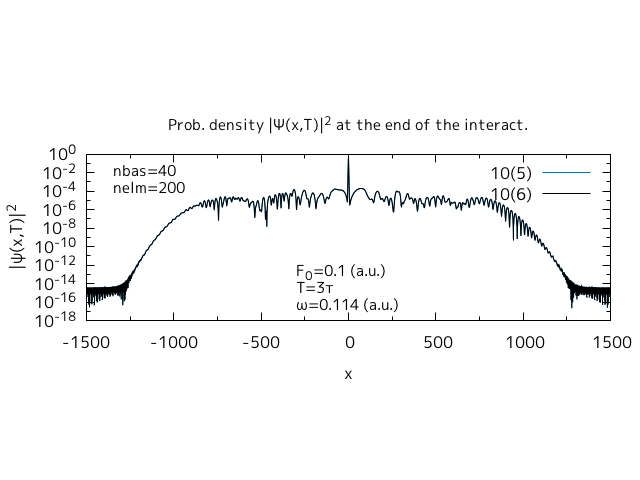
\includegraphics[scale=.20, trim={6 100 10 133},clip]{images/114_f01_3_density_comp.png} \\
 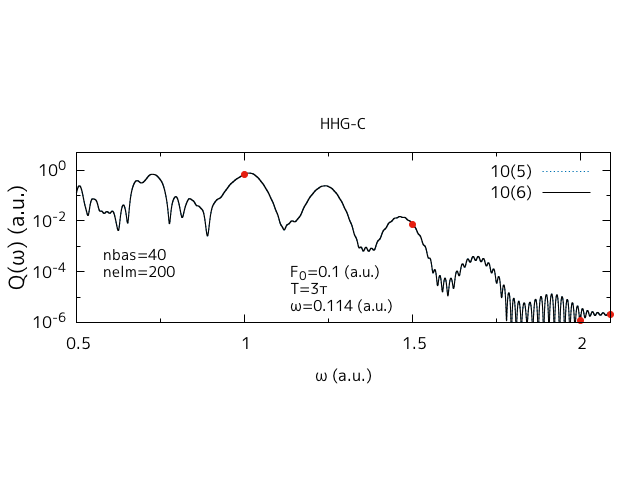
\includegraphics[scale=.20, trim={6 100 10 130},clip]{images/114_f01_3_hhg_comp.png} \\
% \includegraphics[scale=.20, trim={6 130 10 130},clip]{images/114_f003_8_03_hhg.png} 
%%\caption{Eigenvalues.}
%\label{fig:pemd_0114}
 \end{figure}

\end{minipage}
\end{textblock*}


\begin{textblock*}{500pt}(130pt,60pt)
%\centering
%\rotatebox{90}{
 \begin{minipage}{0.0\linewidth}
 \begin{figure}[tp]
 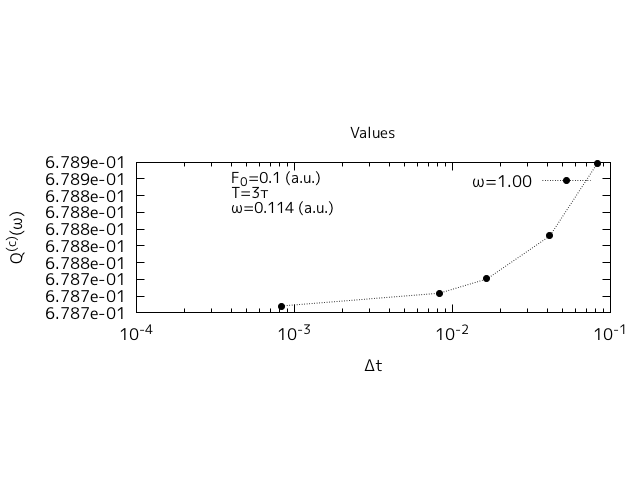
\includegraphics[scale=.20, trim={6 100 10 133},clip]{images/114_f01_3_values_100.png} \\
 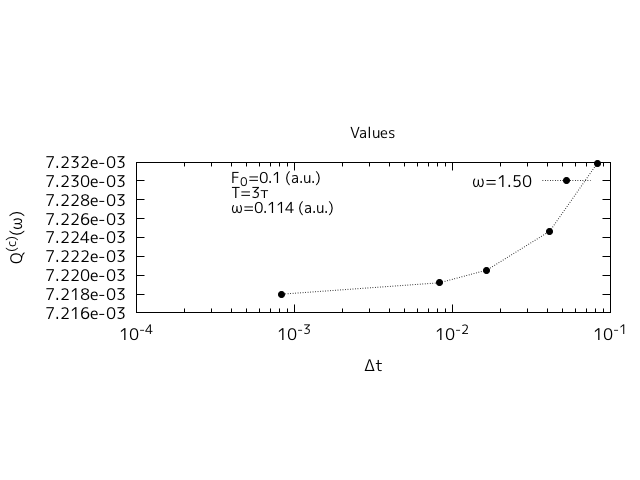
\includegraphics[scale=.20, trim={6 100 10 130},clip]{images/114_f01_3_values_150.png} \\
% 
\includegraphics[scale=.20, trim={30 130 10 130},clip]{images/114_f003_12_07_hhg.png} 
%%\caption{Eigenvalues.}
%\label{fig:pemd_0114}
 \end{figure}

\end{minipage}
\end{textblock*}


\begin{textblock*}{500pt}(255pt,60pt)
%\centering
%\rotatebox{90}{
 \begin{minipage}{0.0\linewidth}
 \begin{figure}[tp]
 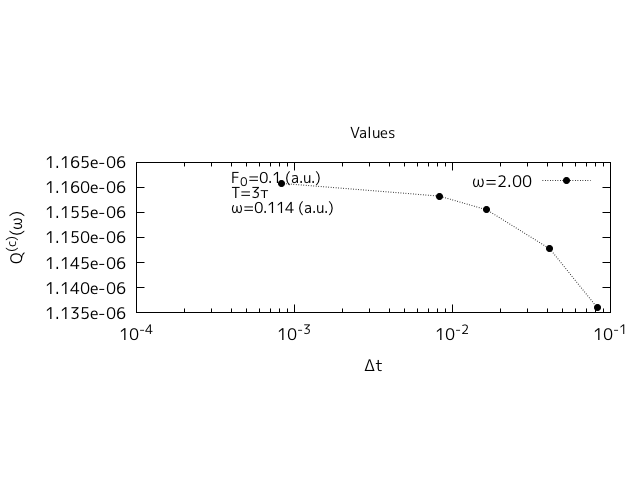
\includegraphics[scale=.20, trim={6 100 10 133},clip]{images/114_f01_3_values_200.png} \\
 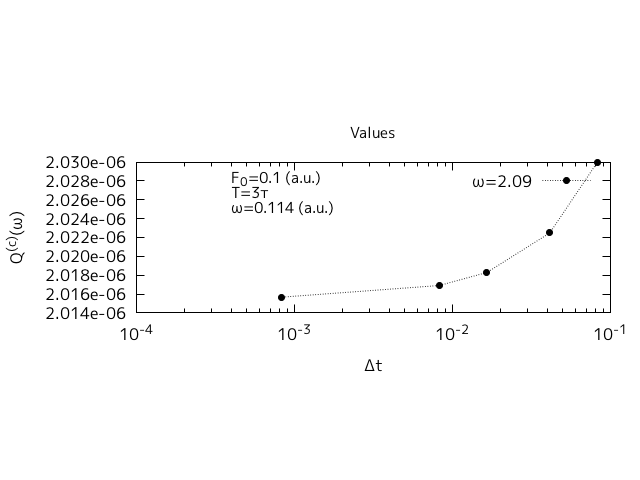
\includegraphics[scale=.20, trim={6 100 10 130},clip]{images/114_f01_3_values_209.png} \\
% 
\includegraphics[scale=.20, trim={30 130 10 130},clip]{images/114_f003_12_07_hhg.png} 
%%\caption{Eigenvalues.}
%\label{fig:pemd_0114}
 \end{figure}

\end{minipage}
\end{textblock*}


\begin{textblock*}{500pt}(390pt,165pt)
%\centering
\rotatebox{90}{
 \begin{minipage}{0.0\linewidth}
 \begin{figure}[tp]
 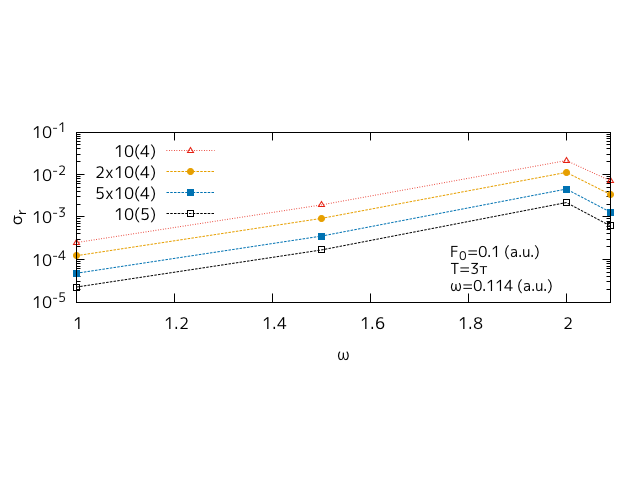
\includegraphics[scale=.20, trim={6 100 10 120},clip]{images/114_f01_3_error.png } \\
%%\caption{Eigenvalues.}
%\label{fig:pemd_0114}
 \end{figure}
\end{minipage}
}
\end{textblock*}




\begin{textblock*}{\linewidth}(20pt,170pt)
\rotatebox{0}{
\begin{minipage}{\linewidth}
{
\tiny 
\centering
\input{tables/114_f01_3t_error_2.tab}
}
\end{minipage}
}
\end{textblock*}


\begin{textblock*}{400pt}(30pt,205pt)
\scriptsize

\begin{align}
    \sigma_{ij}= \left|\frac{\left(   Q^{(c)}(\omega)[i] 
       - Q^{(c)}(\omega)[j]  \right)}{Q^{(c)}(\omega)[j]}\right|, \hspace{20pt}
    Q^{(c)}(\omega) & = \left|\Bigg[ e^{i\omega t} x(t)\Bigg]_{-T/2}^{T/2}
               -i\omega \int_{-T/2}^{T/2} e^{i\omega t}x(t)dt\right|^2.
                \nonumber
\end{align}

\end{textblock*}

\end{frame}






\begin{frame}
\frametitle{Quantum theory of radiation by nonstationary systems 
	with application to high-order harmonic generation
        (Phys. Rev. A 101, 013410 (2020))}
	\framesubtitle{Time dependence - $T=5\tau$}
\small
\begin{textblock*}{500pt}(5pt,60pt)
%\centering
%\rotatebox{90}{
 \begin{minipage}{0.0\linewidth}
 \begin{figure}[tp]
 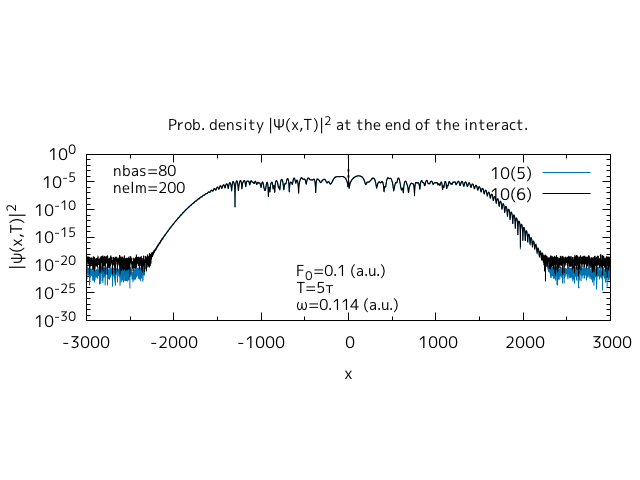
\includegraphics[scale=.20, trim={6 100 10 133},clip]{images/114_f01_5_density_comp.png} \\
 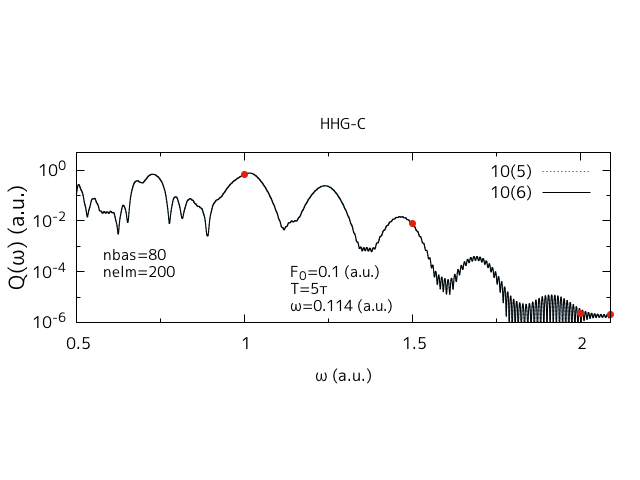
\includegraphics[scale=.20, trim={6 100 10 130},clip]{images/114_f01_5_hhg_comp.png} \\
% \includegraphics[scale=.20, trim={6 130 10 130},clip]{images/114_f003_8_03_hhg.png} 
%%\caption{Eigenvalues.}
%\label{fig:pemd_0114}
 \end{figure}

\end{minipage}
\end{textblock*}


\begin{textblock*}{500pt}(130pt,60pt)
%\centering
%\rotatebox{90}{
 \begin{minipage}{0.0\linewidth}
 \begin{figure}[tp]
 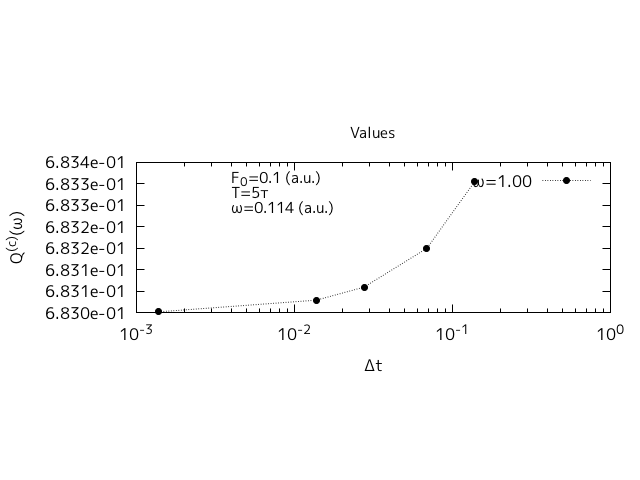
\includegraphics[scale=.20, trim={6 100 10 133},clip]{images/114_f01_5_values_100.png} \\
 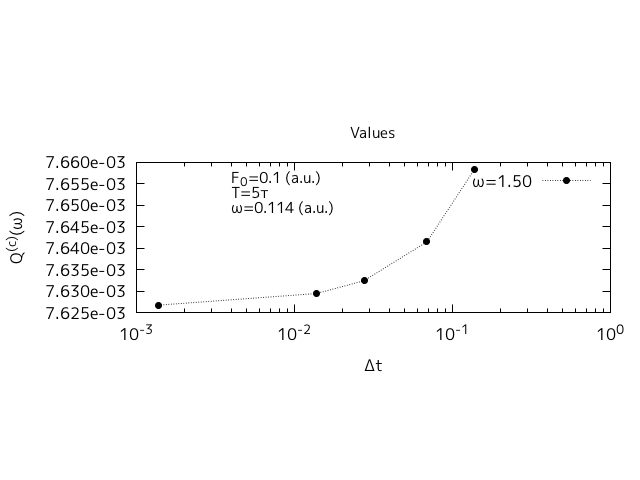
\includegraphics[scale=.20, trim={6 100 10 130},clip]{images/114_f01_5_values_150.png} \\
% 
\includegraphics[scale=.20, trim={30 130 10 130},clip]{images/114_f003_12_07_hhg.png} 
%%\caption{Eigenvalues.}
%\label{fig:pemd_0114}
 \end{figure}

\end{minipage}
\end{textblock*}


\begin{textblock*}{500pt}(255pt,60pt)
%\centering
%\rotatebox{90}{
 \begin{minipage}{0.0\linewidth}
 \begin{figure}[tp]
 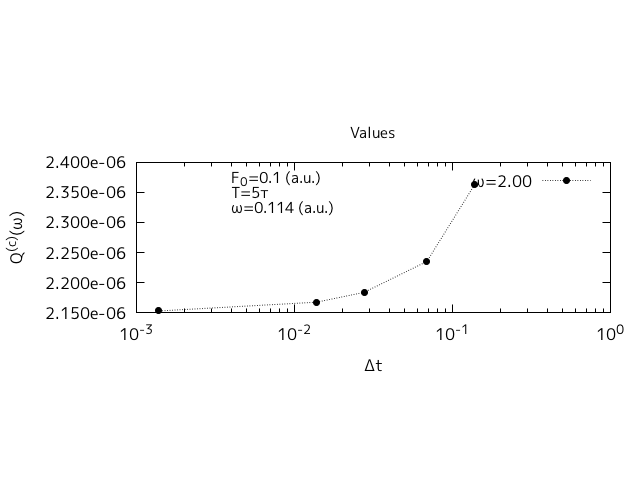
\includegraphics[scale=.20, trim={6 100 10 133},clip]{images/114_f01_5_values_200.png} \\
 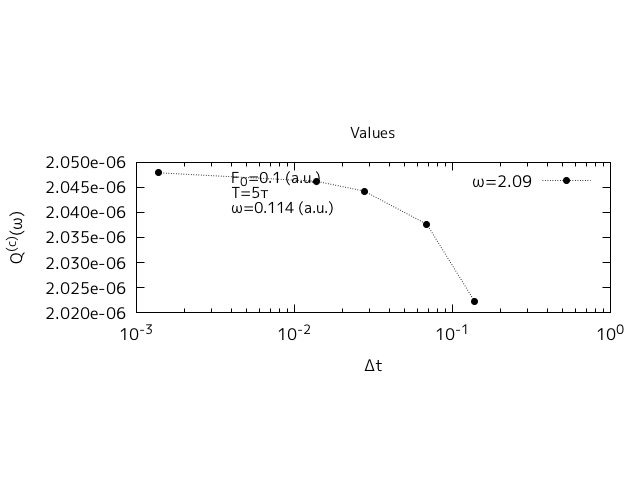
\includegraphics[scale=.20, trim={6 100 10 130},clip]{images/114_f01_5_values_209.png} \\
% 
\includegraphics[scale=.20, trim={30 130 10 130},clip]{images/114_f003_12_07_hhg.png} 
%%\caption{Eigenvalues.}
%\label{fig:pemd_0114}
 \end{figure}

\end{minipage}
\end{textblock*}


\begin{textblock*}{500pt}(390pt,165pt)
%\centering
\rotatebox{90}{
 \begin{minipage}{0.0\linewidth}
 \begin{figure}[tp]
 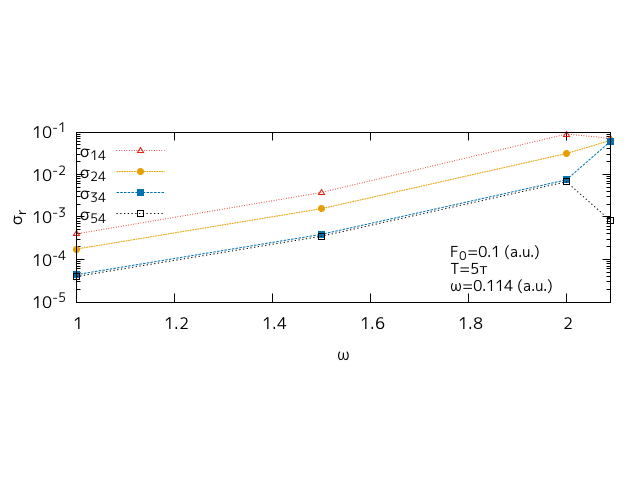
\includegraphics[scale=.20, trim={6 100 10 132},clip]{images/114_f01_5_error.png } \\
%%\caption{Eigenvalues.}
%\label{fig:pemd_0114}
 \end{figure}
\end{minipage}
}
\end{textblock*}




\begin{textblock*}{\linewidth}(20pt,170pt)
\rotatebox{0}{
\begin{minipage}{\linewidth}
{
\tiny 
\centering
\input{tables/114_f01_5t_error_2.tab}
}
\end{minipage}
}
\end{textblock*}


\begin{textblock*}{400pt}(30pt,205pt)
\scriptsize

\begin{align}
    \sigma_{ij} = \left|\frac{\left(   Q^{(c)}(\omega)[i] 
       - Q^{(c)}(\omega)[j]  \right)}{Q^{(c)}(\omega)[j]}\right|, \hspace{20pt}
    Q^{(c)}(\omega) & = \left|\Bigg[ e^{i\omega t} x(t)\Bigg]_{-T/2}^{T/2}
               -i\omega \int_{-T/2}^{T/2} e^{i\omega t}x(t)dt\right|^2.
                \nonumber
\end{align}

\end{textblock*}

\end{frame}





\begin{frame}
\frametitle{Quantum theory of radiation by nonstationary systems 
	with application to high-order harmonic generation
        (Phys. Rev. A 101, 013410 (2020))}
	\framesubtitle{Time dependence - $T=8\tau$}
\small
\begin{textblock*}{500pt}(5pt,60pt)
%\centering
%\rotatebox{90}{
 \begin{minipage}{0.0\linewidth}
 \begin{figure}[tp]
 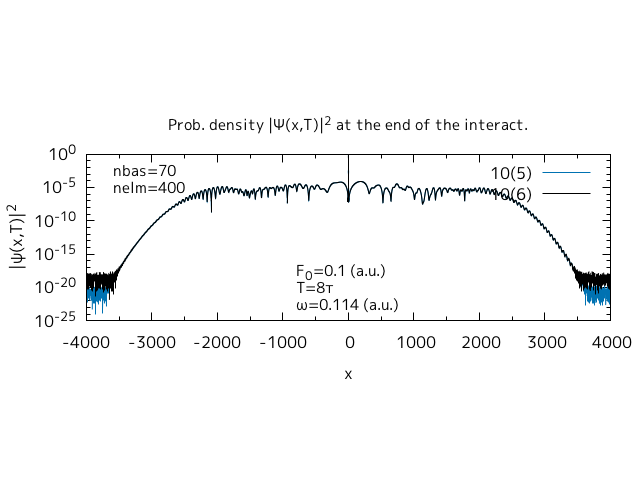
\includegraphics[scale=.20, trim={6 100 10 133},clip]{images/114_f01_8_density_comp.png} \\
 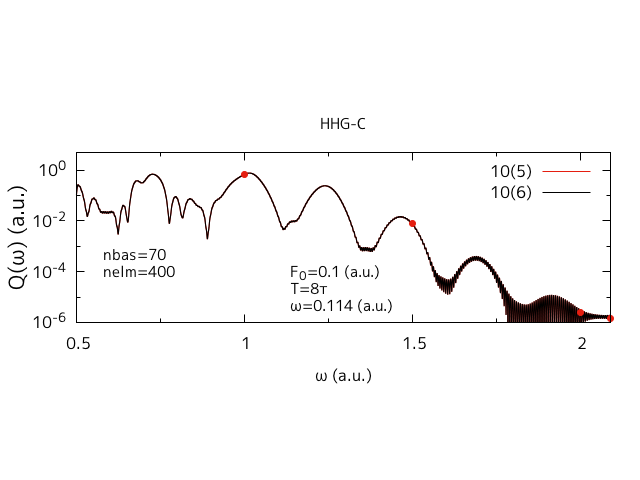
\includegraphics[scale=.20, trim={6 100 10 130},clip]{images/114_f01_8_hhg_comp.png} \\
% \includegraphics[scale=.20, trim={6 130 10 130},clip]{images/114_f003_8_03_hhg.png} 
%%\caption{Eigenvalues.}
%\label{fig:pemd_0114}
 \end{figure}

\end{minipage}
\end{textblock*}


\begin{textblock*}{500pt}(130pt,60pt)
%\centering
%\rotatebox{90}{
 \begin{minipage}{0.0\linewidth}
 \begin{figure}[tp]
 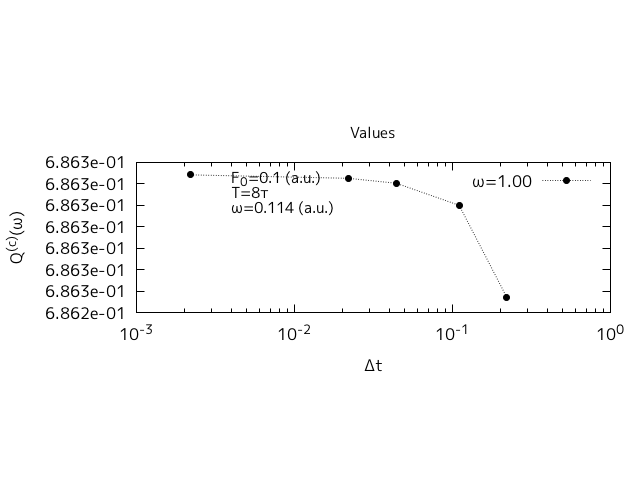
\includegraphics[scale=.20, trim={6 100 10 133},clip]{images/114_f01_8_values_100.png} \\
 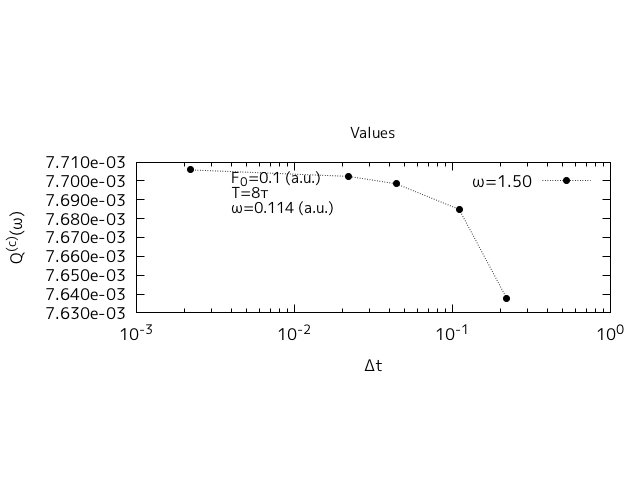
\includegraphics[scale=.20, trim={6 100 10 130},clip]{images/114_f01_8_values_150.png} \\
% 
\includegraphics[scale=.20, trim={30 130 10 130},clip]{images/114_f003_12_07_hhg.png} 
%%\caption{Eigenvalues.}
%\label{fig:pemd_0114}
 \end{figure}

\end{minipage}
\end{textblock*}


\begin{textblock*}{500pt}(255pt,60pt)
%\centering
%\rotatebox{90}{
 \begin{minipage}{0.0\linewidth}
 \begin{figure}[tp]
 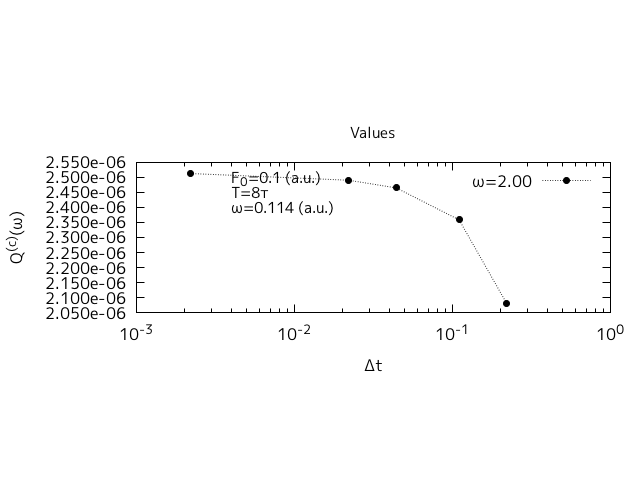
\includegraphics[scale=.20, trim={6 100 10 133},clip]{images/114_f01_8_values_200.png} \\
 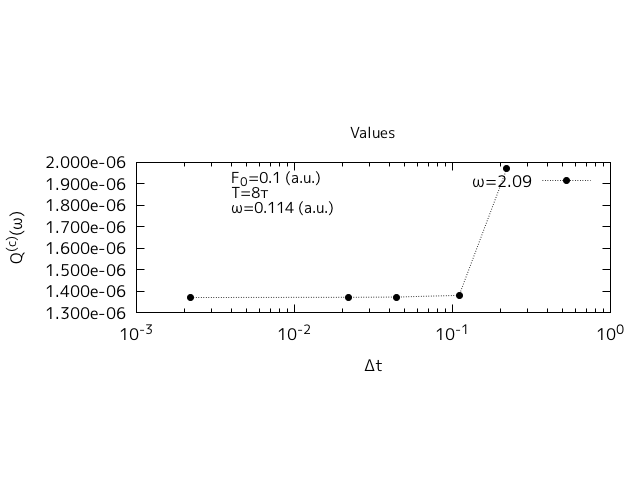
\includegraphics[scale=.20, trim={6 100 10 130},clip]{images/114_f01_8_values_209.png} \\
% 
\includegraphics[scale=.20, trim={30 130 10 130},clip]{images/114_f003_12_07_hhg.png} 
%%\caption{Eigenvalues.}
%\label{fig:pemd_0114}
 \end{figure}

\end{minipage}
\end{textblock*}


\begin{textblock*}{500pt}(390pt,165pt)
%\centering
\rotatebox{90}{
 \begin{minipage}{0.0\linewidth}
 \begin{figure}[tp]
 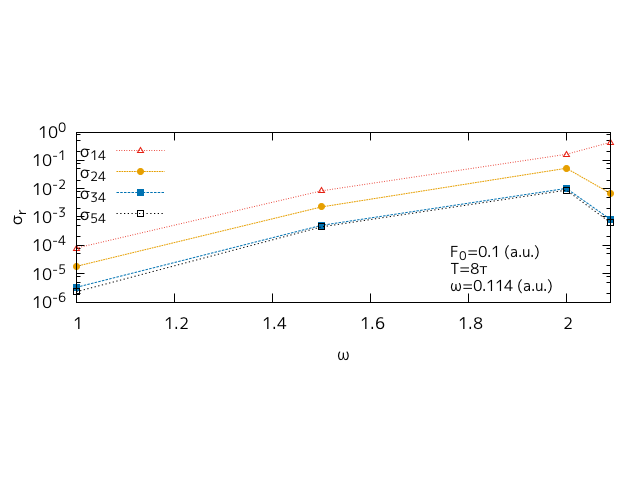
\includegraphics[scale=.20, trim={6 100 10 120},clip]{images/114_f01_8_error.png } \\
%%\caption{Eigenvalues.}
%\label{fig:pemd_0114}
 \end{figure}
\end{minipage}
}
\end{textblock*}




\begin{textblock*}{\linewidth}(20pt,170pt)
\rotatebox{0}{
\begin{minipage}{\linewidth}
{
\tiny 
\centering
\input{tables/114_f01_8t_error_2.tab}
}
\end{minipage}
}
\end{textblock*}


\begin{textblock*}{400pt}(30pt,205pt)
\scriptsize

\begin{align}
    \sigma_{ij} = \left|\frac{\left(   Q^{(c)}(\omega)[i] 
       - Q^{(c)}(\omega) [j] \right)}{Q^{(c)}(\omega)[j]}\right|, \hspace{20pt}
    Q^{(c)}(\omega) & = \left|\Bigg[ e^{i\omega t} x(t)\Bigg]_{-T/2}^{T/2}
               -i\omega \int_{-T/2}^{T/2} e^{i\omega t}x(t)dt\right|^2.
                \nonumber
\end{align}

\end{textblock*}

\end{frame}



\begin{frame}
\frametitle{Quantum theory of radiation by nonstationary systems 
	with application to high-order harmonic generation
        (Phys. Rev. A 101, 013410 (2020))}
	\framesubtitle{Time dependence reference table}
\small

\begin{textblock*}{400pt}(30pt,60pt)
\footnotesize
\begin{itemize}
\item Sufficient time step for converged result is 
$\Delta t \leqslant 0.08\,\rm a.u.$
\item In the following, we will maintain $\Delta t$ set to 
around $0.04\,\rm a.u.$
\end{itemize}

\end{textblock*}

{
\tiny 
\input{tables/ref_dt.tab}
}


\begin{textblock*}{400pt}(30pt,205pt)
\scriptsize

\begin{align}
    \tau = n_{oc}\frac{2\pi}{\omega}, \hspace{20pt}
    T = n \tau, \hspace{20pt}
    \Delta t  = \frac{T}{{\rm nsteps}}, \hspace{20pt}
    n_{oc}  = 5,
                \nonumber
\end{align}

\end{textblock*}

\end{frame}




%\begin{frame}
%\frametitle{Quantum theory of radiation by nonstationary systems 
%	with application to high-order harmonic generation
%        (Phys. Rev. A 101, 013410 (2020))}
%	\framesubtitle{Time dependence - $\rm{nsteps} = 100000$}
%\small
%\begin{textblock*}{500pt}(5pt,60pt)
%%\centering
%%\rotatebox{90}{
% \begin{minipage}{0.0\linewidth}
% \begin{figure}[tp]
% 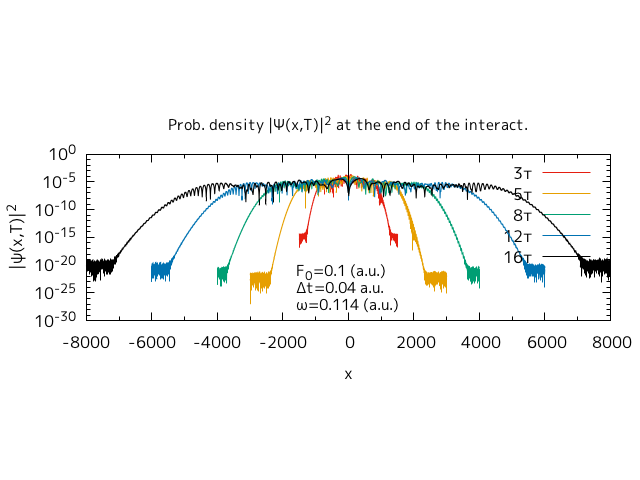
\includegraphics[scale=.20, trim={6 100 10 133},clip]{images/114_f01_T_density_comp.png} \\
% 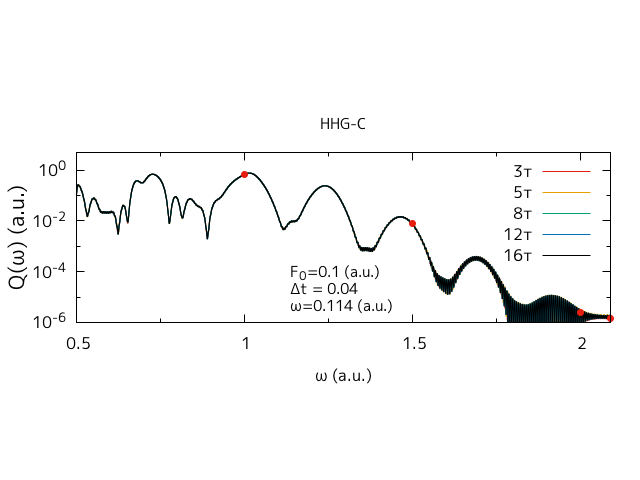
\includegraphics[scale=.20, trim={6 100 10 130},clip]{images/114_f01_T_hhg_comp.png} \\
%% \includegraphics[scale=.20, trim={6 130 10 130},clip]{images/114_f003_8_03_hhg.png} 
%%%\caption{Eigenvalues.}
%%\label{fig:pemd_0114}
% \end{figure}
%
%\end{minipage}
%\end{textblock*}
%
%
%\begin{textblock*}{500pt}(130pt,60pt)
%%\centering
%%\rotatebox{90}{
% \begin{minipage}{0.0\linewidth}
% \begin{figure}[tp]
% \includegraphics[scale=.20, trim={6 100 10 133},clip]{images/114_f01_T_values_100.png} \\
% \includegraphics[scale=.20, trim={6 100 10 130},clip]{images/114_f01_T_values_150.png} \\
%% 
\includegraphics[scale=.20, trim={30 130 10 130},clip]{images/114_f003_12_07_hhg.png} 
%%%\caption{Eigenvalues.}
%%\label{fig:pemd_0114}
% \end{figure}
%
%\end{minipage}
%\end{textblock*}
%
%
%\begin{textblock*}{500pt}(255pt,60pt)
%%\centering
%%\rotatebox{90}{
% \begin{minipage}{0.0\linewidth}
% \begin{figure}[tp]
% \includegraphics[scale=.20, trim={6 100 10 133},clip]{images/114_f01_T_values_200.png} \\
% \includegraphics[scale=.20, trim={6 100 10 130},clip]{images/114_f01_T_values_209.png} \\
%% 
\includegraphics[scale=.20, trim={30 130 10 130},clip]{images/114_f003_12_07_hhg.png} 
%%%\caption{Eigenvalues.}
%%\label{fig:pemd_0114}
% \end{figure}
%
%\end{minipage}
%\end{textblock*}
%
%
%%\begin{textblock*}{500pt}(390pt,165pt)
%%%\centering
%%\rotatebox{90}{
%% \begin{minipage}{0.0\linewidth}
%% \begin{figure}[tp]
%% 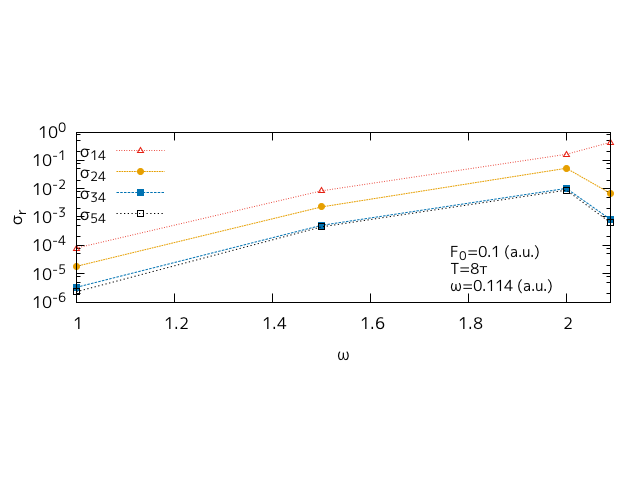
\includegraphics[scale=.20, trim={6 100 10 120},clip]{images/114_f01_8_error.png } \\
%%%%\caption{Eigenvalues.}
%%%\label{fig:pemd_0114}
%% \end{figure}
%%\end{minipage}
%%}
%%\end{textblock*}
%
%
%
%
%\begin{textblock*}{\linewidth}(20pt,170pt)
%\rotatebox{0}{
%\begin{minipage}{\linewidth}
%{
%\tiny 
%\centering
%\input{tables/114_f01_T_100000.tab}
%}
%\end{minipage}
%}
%\end{textblock*}
%
%
%\begin{textblock*}{400pt}(30pt,205pt)
%\scriptsize
%
%\begin{align}
%%   \sigma_{ij} = \left|\frac{\left(   Q^{(c)}(\omega)[i] 
%%      - Q^{(c)}(\omega) [j] \right)}{Q^{(c)}(\omega)[j]}\right|, \hspace{20pt}
%    Q^{(c)}(\omega) & = \left|\Bigg[ e^{i\omega t} x(t)\Bigg]_{-T/2}^{T/2}
%               -i\omega \int_{-T/2}^{T/2} e^{i\omega t}x(t)dt\right|^2.
%                \nonumber
%\end{align}
%
%\end{textblock*}
%
%\end{frame}










\begin{frame}
\frametitle{Quantum theory of radiation by nonstationary systems 
	with application to high-order harmonic generation
        (Phys. Rev. A 101, 013410 (2020))}
	\framesubtitle{Time dependence - $F_0 = 0.1\,{\rm a.u.}\;\;
                          \Delta t= 0.04\,\rm a.u.$}
\small
\begin{textblock*}{500pt}(5pt,60pt)
%\centering
%\rotatebox{90}{
 \begin{minipage}{0.0\linewidth}
 \begin{figure}[tp]
 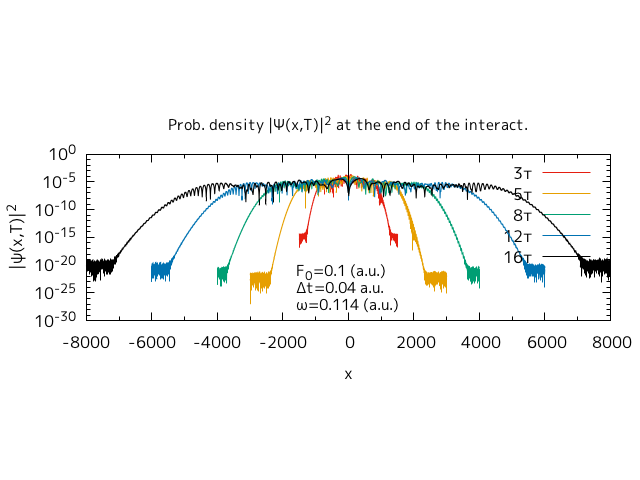
\includegraphics[scale=.20, trim={6 100 10 133},clip]{images/114_f01_T_density_comp.png} \\
 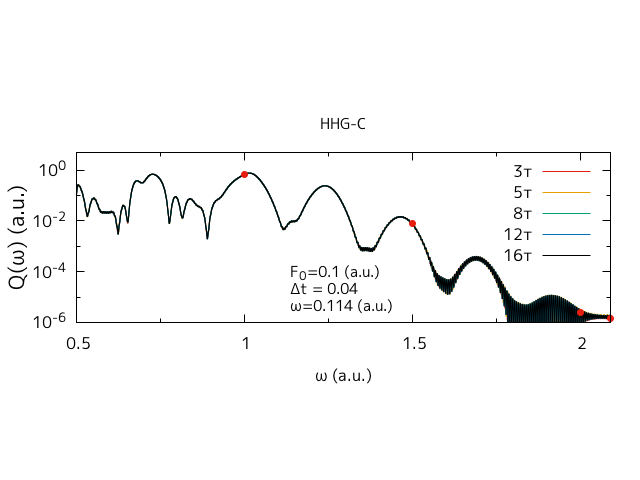
\includegraphics[scale=.20, trim={6 100 10 130},clip]{images/114_f01_T_hhg_comp.png} \\
% \includegraphics[scale=.20, trim={6 130 10 130},clip]{images/114_f003_8_03_hhg.png} 
%%\caption{Eigenvalues.}
%\label{fig:pemd_0114}
 \end{figure}

\end{minipage}
\end{textblock*}


\begin{textblock*}{500pt}(130pt,60pt)
%\centering
%\rotatebox{90}{
 \begin{minipage}{0.0\linewidth}
 \begin{figure}[tp]
 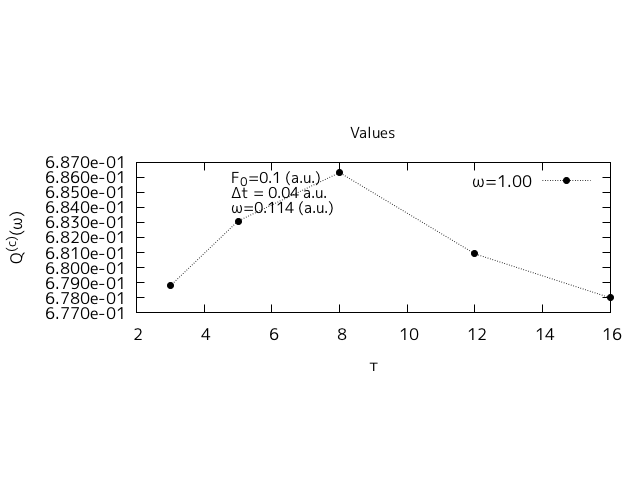
\includegraphics[scale=.20, trim={6 100 10 133},clip]{images/114_f01_T_values_dt_100.png} \\
 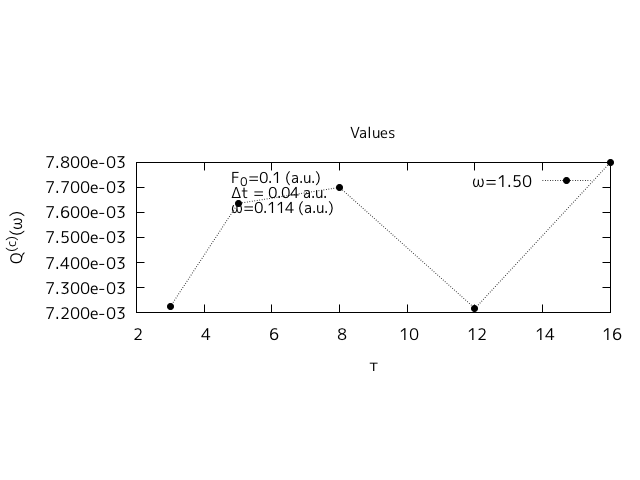
\includegraphics[scale=.20, trim={6 100 10 130},clip]{images/114_f01_T_values_dt_150.png} \\
% 
\includegraphics[scale=.20, trim={30 130 10 130},clip]{images/114_f003_12_07_hhg.png} 
%%\caption{Eigenvalues.}
%\label{fig:pemd_0114}
 \end{figure}

\end{minipage}
\end{textblock*}


\begin{textblock*}{500pt}(255pt,60pt)
%\centering
%\rotatebox{90}{
 \begin{minipage}{0.0\linewidth}
 \begin{figure}[tp]
 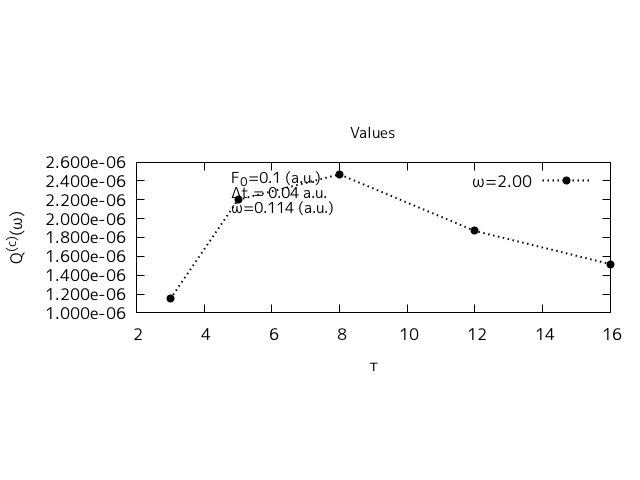
\includegraphics[scale=.20, trim={6 100 10 133},clip]{images/114_f01_T_values_dt_200.png} \\
 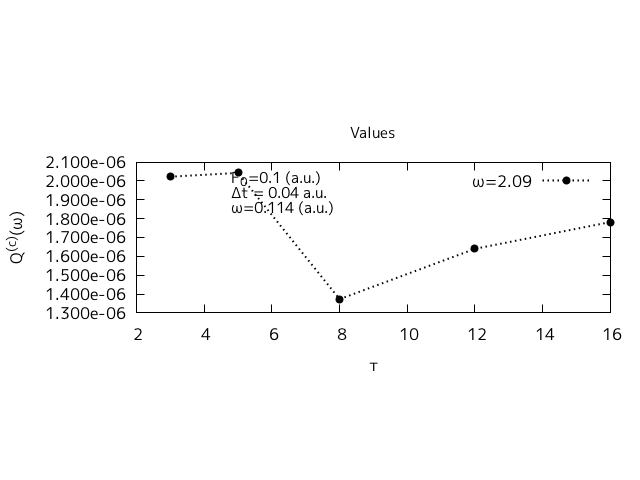
\includegraphics[scale=.20, trim={6 100 10 130},clip]{images/114_f01_T_values_dt_209.png} \\
% 
\includegraphics[scale=.20, trim={30 130 10 130},clip]{images/114_f003_12_07_hhg.png} 
%%\caption{Eigenvalues.}
%\label{fig:pemd_0114}
 \end{figure}

\end{minipage}
\end{textblock*}


%\begin{textblock*}{500pt}(390pt,165pt)
%%\centering
%\rotatebox{90}{
% \begin{minipage}{0.0\linewidth}
% \begin{figure}[tp]
% 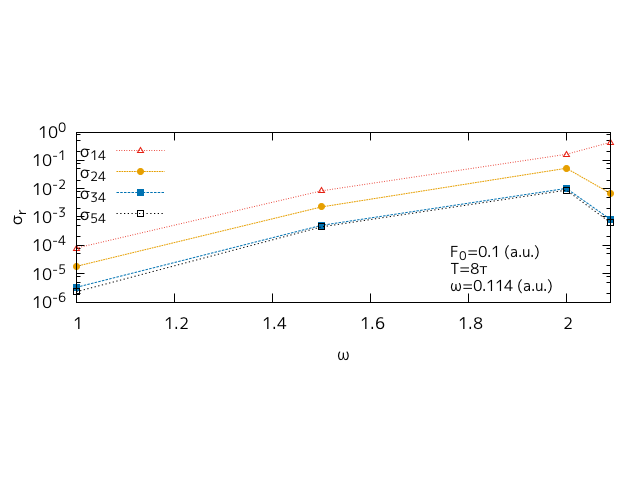
\includegraphics[scale=.20, trim={6 100 10 120},clip]{images/114_f01_8_error.png } \\
%%%\caption{Eigenvalues.}
%%\label{fig:pemd_0114}
% \end{figure}
%\end{minipage}
%}
%\end{textblock*}




\begin{textblock*}{\linewidth}(20pt,170pt)
\rotatebox{0}{
\begin{minipage}{\linewidth}
{
\tiny 
\centering
\input{tables/114_f01_T_dt004.tab}
}
\end{minipage}
}
\end{textblock*}


\begin{textblock*}{400pt}(30pt,215pt)
\scriptsize

\begin{align}
%   \sigma_{ij} = \left|\frac{\left(   Q^{(c)}(\omega)[i] 
%      - Q^{(c)}(\omega) [j] \right)}{Q^{(c)}(\omega)[j]}\right|, \hspace{20pt}
    Q^{(c)}(\omega) & = \left|\Bigg[ e^{i\omega t} x(t)\Bigg]_{-T/2}^{T/2}
               -i\omega \int_{-T/2}^{T/2} e^{i\omega t}x(t)dt\right|^2.
                \nonumber
\end{align}

\end{textblock*}

\end{frame}




\begin{frame}
\frametitle{Quantum theory of radiation by nonstationary systems 
	with application to high-order harmonic generation
        (Phys. Rev. A 101, 013410 (2020))}
	\framesubtitle{Time dependence - $F_0 = 0.3\,{\rm a.u.}\;\;
                          \Delta t= 0.04\,\rm a.u.$}
\small
\begin{textblock*}{500pt}(5pt,60pt)
%\centering
%\rotatebox{90}{
 \begin{minipage}{0.0\linewidth}
 \begin{figure}[tp]
%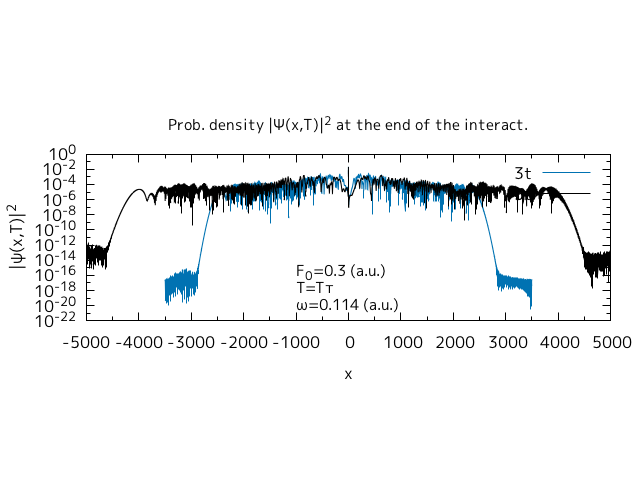
\includegraphics[scale=.20, trim={6 100 10 133},clip]{images/114_f03_T_density_comp.png} \\
% \includegraphics[scale=.20, trim={6 100 10 130},clip]{images/114_f03_T_hhg_comp.png} \\
%% \includegraphics[scale=.20, trim={6 130 10 130},clip]{images/114_f003_8_03_hhg.png} 
%%\caption{Eigenvalues.}
%\label{fig:pemd_0114}
 \end{figure}

\end{minipage}
\end{textblock*}


%\begin{textblock*}{500pt}(130pt,60pt)
%%\centering
%%\rotatebox{90}{
% \begin{minipage}{0.0\linewidth}
% \begin{figure}[tp]
% 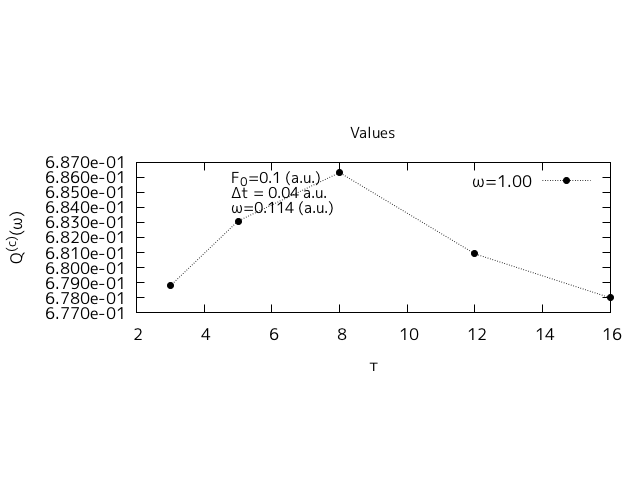
\includegraphics[scale=.20, trim={6 100 10 133},clip]{images/114_f01_T_values_dt_100.png} \\
% 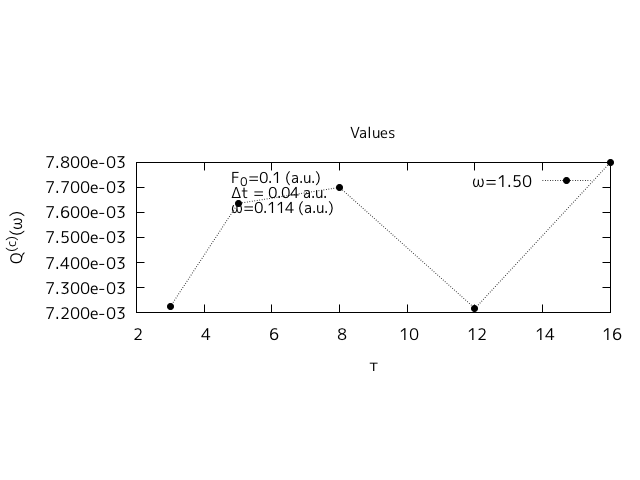
\includegraphics[scale=.20, trim={6 100 10 130},clip]{images/114_f01_T_values_dt_150.png} \\
%% 
\includegraphics[scale=.20, trim={30 130 10 130},clip]{images/114_f003_12_07_hhg.png} 
%%%\caption{Eigenvalues.}
%%\label{fig:pemd_0114}
% \end{figure}
%
%\end{minipage}
%\end{textblock*}
%
%
%\begin{textblock*}{500pt}(255pt,60pt)
%%\centering
%%\rotatebox{90}{
% \begin{minipage}{0.0\linewidth}
% \begin{figure}[tp]
% 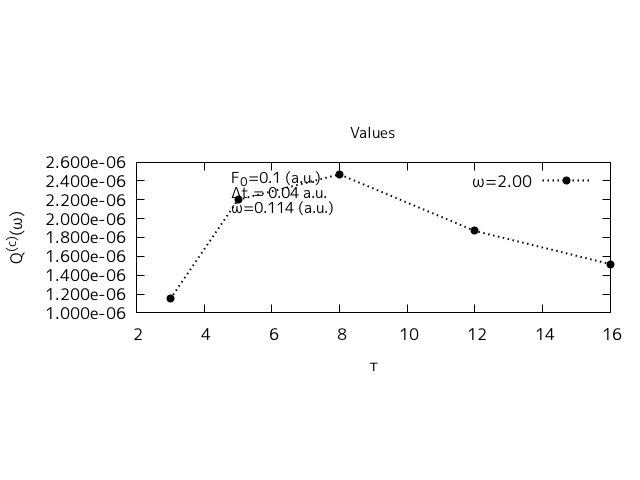
\includegraphics[scale=.20, trim={6 100 10 133},clip]{images/114_f01_T_values_dt_200.png} \\
% 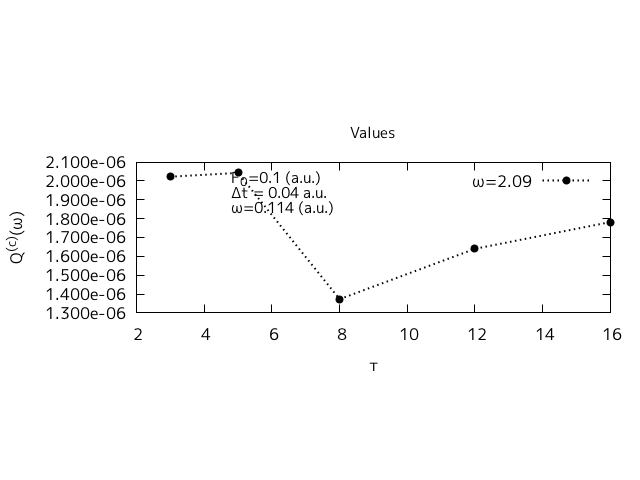
\includegraphics[scale=.20, trim={6 100 10 130},clip]{images/114_f01_T_values_dt_209.png} \\
%% 
\includegraphics[scale=.20, trim={30 130 10 130},clip]{images/114_f003_12_07_hhg.png} 
%%%\caption{Eigenvalues.}
%%\label{fig:pemd_0114}
% \end{figure}
%
%\end{minipage}
%\end{textblock*}
%
%
%%\begin{textblock*}{500pt}(390pt,165pt)
%%%\centering
%%\rotatebox{90}{
%% \begin{minipage}{0.0\linewidth}
%% \begin{figure}[tp]
%% 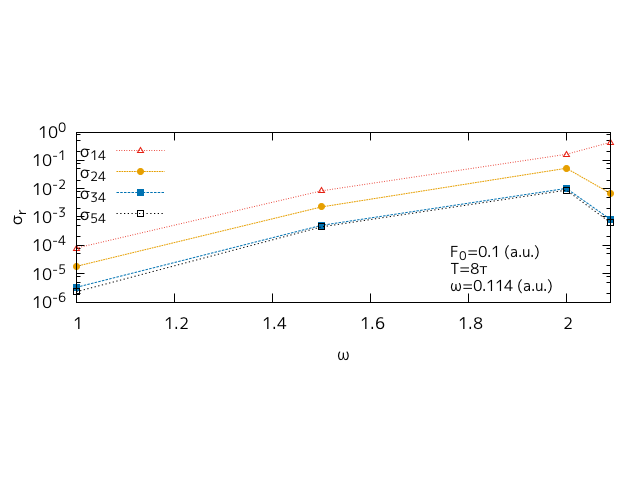
\includegraphics[scale=.20, trim={6 100 10 120},clip]{images/114_f01_8_error.png } \\
%%%%\caption{Eigenvalues.}
%%%\label{fig:pemd_0114}
%% \end{figure}
%%\end{minipage}
%%}
%%\end{textblock*}
%
%


\begin{textblock*}{\linewidth}(20pt,170pt)
\rotatebox{0}{
\begin{minipage}{\linewidth}
{
\tiny 
\centering
\input{tables/114_f03_T_dt004.tab}
}
\end{minipage}
}
\end{textblock*}


\begin{textblock*}{400pt}(30pt,215pt)
\scriptsize

\begin{align}
%   \sigma_{ij} = \left|\frac{\left(   Q^{(c)}(\omega)[i] 
%      - Q^{(c)}(\omega) [j] \right)}{Q^{(c)}(\omega)[j]}\right|, \hspace{20pt}
    Q^{(c)}(\omega) & = \left|\Bigg[ e^{i\omega t} x(t)\Bigg]_{-T/2}^{T/2}
               -i\omega \int_{-T/2}^{T/2} e^{i\omega t}x(t)dt\right|^2.
                \nonumber
\end{align}

\end{textblock*}

\end{frame}




\begin{frame}
\frametitle{Quantum theory of radiation by nonstationary systems 
	with application to high-order harmonic generation
        (Phys. Rev. A 101, 013410 (2020))}
	\framesubtitle{Convergence parameters table for 
             the homogeneous equation}
\small

\begin{textblock*}{400pt}(30pt,60pt)
\footnotesize
\begin{itemize}
\item The following table shows parameters known to return converged results 
for Eq. (\ref{eqn:step_1d}), which is recalled below
%\item \textbf{For $\omega=0.057\,\rm a.u.$ and $F_0 = 0.3\,\rm a.u.$,
%PEMD and HHG spectra currently do not converge even 
%when density probability does}
\end{itemize}

\end{textblock*}

\vspace{20pt}

{
\tiny 
\input{tables/conv_table_057.tab}
\input{tables/conv_table_114.tab}
}


\begin{textblock*}{400pt}(30pt,205pt)
\scriptsize

\begin{equation}
	i\frac{\partial}{\partial t}\psi(x,t)
	   = \left( \hat{H}_a + \hat{V}_{\rm ext}(t)\right) 
	   \psi(x,t),   \hspace{20pt}\psi(x,0)=\psi_0(x), \nonumber
\end{equation}
\begin{equation}
  \hat{H}_a = -\frac{1}{2}\frac{d^2}{dx^2} - \varkappa\delta(x), \hspace{20pt}
  \hat{V}_{\rm ext} = F(t)x,   \nonumber
\end{equation}

\end{textblock*}


\begin{textblock*}{100pt}(30pt,140pt)
\scriptsize
\textbf{Legend} \\
$\rm (nbas/nelm) - xmax $


\end{textblock*}

\end{frame}



\begin{frame}
\frametitle{Quantum theory of radiation by nonstationary systems 
	with application to high-order harmonic generation
        (Phys. Rev. A 101, 013410 (2020))}
	\framesubtitle{Structure of the code, performance 
         and memory management}
\small

\begin{textblock*}{400pt}(30pt,60pt)
\footnotesize
\begin{enumerate}
\item Diagonalization
\begin{itemize}
\footnotesize
\item[$\bullet$] most time consuming part for bigger matrixes
\item[$\bullet$] is there a way to multithread lapack diagonalization? 
\end{itemize}
\item Propagation
\begin{itemize}
\footnotesize
\item[$\bullet$] can be arbitrarily long 
(convergence requires $\Delta t \leqslant 0.08\,\rm a.u.$)
\item[$\bullet$] order 4 scheme required
\item[$\bullet$] multithreading would also help here
\end{itemize}
\item Projection 
\begin{itemize}
\footnotesize
\item[$\bullet$] very short (matter of minutes)
\item[$\bullet$] potentially very memory consuming
\end{itemize}
\end{enumerate}

\vspace{10pt}

1. and 2. take some memory for a long time, 
3. takes even more memory for a very short time. \\
Any run for large matrixes required to split those processes.


\end{textblock*}

\end{frame}



\begin{frame}
\frametitle{Quantum theory of radiation by nonstationary systems 
	with application to high-order harmonic generation
        (Phys. Rev. A 101, 013410 (2020))}
	\framesubtitle{Numerical toolkit - 1}
\small

\begin{textblock*}{400pt}(30pt,60pt)
\footnotesize
\begin{itemize}
\item Integration is done by using the following order 2 methods
\begin{itemize}
\item[$\bullet$] the (1/3) Simpson rule,
$m$ being the number of subintervals
%with $h=(x_{m}-x_0)/m$, $x_i = x_0 + ih$,
\begin{align}
\begin{split}
 \int_{x_0}^{x_m} f(x)dx & \sim \frac{1}{3} h \sum_{i=1}^{m/2}
  \left[ f(x_{2i-2})  + 4f(x_{2i-1}) + f(x_{2i})\right]\;\;\mbox{ (1/3 rule) }
\end{split} \label{eqn:simps18} 
%\begin{split}
% \int_{x_0}^{x_m} f(x)dx & \sim \frac{3}{8} h \sum_{i=1}^{m/3}
%  \left[ f(x_{3i-3})  + 3f(x_{3i-2}) +    \right.
%  \left. 3f(x_{3i-1}) + f(x_{3i})\right]\;\;\mbox{ (3/8 rule) },
%\end{split} \label{eqn:simps38} 
\end{align}

\item[$\bullet$] the trapezoidal rule
\begin{align}
\begin{split}
 \int_{x_0}^{x_m} f(x)dx 
   & \sim \sum_{i=1}^{m} \frac{ f(x_{i-1})  + f(x_{i})}{2}\Delta x_i
\end{split} \label{eqn:trapez} 
\end{align}
\end{itemize}

%\item Numerical differentiation may be done by using the formulas
%
%\begin{align}
%\begin{split}
%f^{\prime}_l (x_i) = \frac{f(x_{i+1}) -  f(x_i)}{x_{i+1} -x_i}, & \hspace{20pt}
%f^{\prime}_r (x_i) = \frac{f(x_{i}) -  f(x_{i-1})}{x_{i} - x_{i-1}}
%\end{split} \label{eqn:diff}   \\
%f^{\prime} (x_i) = & \frac{f^{\prime}_l (x_i) + f^{\prime}_r (x_i)}{2}
%%\begin{split}
%% \int_{x_0}^{x_m} f(x)dx & \sim \frac{3}{8} h \sum_{i=1}^{m/3}
%%  \left[ f(x_{3i-3})  + 3f(x_{3i-2}) +    \right.
%%  \left. 3f(x_{3i-1}) + f(x_{3i})\right]\;\;\mbox{ (3/8 rule) },
%%\end{split} \label{eqn:simps38} 
%\end{align}

\end{itemize}

\end{textblock*}


\end{frame}



%\begin{frame}
%\frametitle{Quantum theory of radiation by nonstationary systems 
%	with application to high-order harmonic generation
%        (Phys. Rev. A 101, 013410 (2020))}
%	\framesubtitle{Numerical toolkit - 2}
%\small
%
%\begin{textblock*}{400pt}(30pt,60pt)
%\footnotesize
%\begin{itemize}
%%\item Integration is done by using the following Simpson rule,
%%$m$ being the number of subintervals
%%with $h=(x_{m}-x_0)/m$, $x_i = x_0 + ih$,
%%\begin{align}
%%\begin{split}
%% \int_{x_0}^{x_m} f(x)dx & \sim \frac{1}{3} h \sum_{i=1}^{m/2}
%%  \left[ f(x_{2i-2})  + 4f(x_{2i-1}) + f(x_{2i})\right]\;\;\mbox{ (1/3 rule) }
%%\end{split} \label{eqn:simps18} 
%%%\begin{split}
%%% \int_{x_0}^{x_m} f(x)dx & \sim \frac{3}{8} h \sum_{i=1}^{m/3}
%%%  \left[ f(x_{3i-3})  + 3f(x_{3i-2}) +    \right.
%%%  \left. 3f(x_{3i-1}) + f(x_{3i})\right]\;\;\mbox{ (3/8 rule) },
%%%\end{split} \label{eqn:simps38} 
%%\end{align}
%%
%%or the trapezoidal rule, given by
%%\begin{align}
%%\begin{split}
%% \int_{x_0}^{x_m} f(x)dx 
%%   & \sim \sum_{i=1}^{m} \frac{ f(x_{i-1})  + f(x_{i})}{2}\Delta x_i
%%\end{split} \label{eqn:trapez} 
%%\end{align}
%
%\item Finite differences
%
%\begin{align}
%\begin{cases}
%f^{\prime}_l (x_i) = \frac{f(x_{i+1}) -  f(x_i)}{x_{i+1} -x_i},  \hspace{20pt}
%f^{\prime}_r (x_i) = \frac{f(x_{i}) -  f(x_{i-1})}{x_{i} - x_{i-1}} \\
%f^{\prime} (x_i) = \frac{f^{\prime}_l (x_i) + f^{\prime}_r (x_i)}{2}
%\end{cases} \label{eqn:diff}  
%%\begin{split}
%% \int_{x_0}^{x_m} f(x)dx & \sim \frac{3}{8} h \sum_{i=1}^{m/3}
%%  \left[ f(x_{3i-3})  + 3f(x_{3i-2}) +    \right.
%%  \left. 3f(x_{3i-1}) + f(x_{3i})\right]\;\;\mbox{ (3/8 rule) },
%%\end{split} \label{eqn:simps38} 
%\end{align}
% 
%\item Using the reciprocal space for differentiating (Fourier transform) 
%\begin{align}
%\hat{f}(k,t) = \int_{-\infty}^{\infty} f(x,t) e^{-ikx}dx,
%\hspace{20pt}\Longrightarrow\hspace{20pt}
%\frac{\partial}{\partial x} f(x,t) 
% = \frac{1}{2\pi}\int_{-\infty}^{\infty} ik\hat{f}(k,t) e^{ikx}dk,
%\label{eqn:diff2}  
%\end{align}
%
%\item Let us also write the dispersion relation
%\begin{align}
%\omega = \frac{k^2}{2}\hspace{20pt} \Longrightarrow \hspace{20pt} 
%k = \pm \sqrt{2\omega}
%\end{align}
%
%\item The delta function is evaluated as
%\begin{align}
%\delta(k-k^\prime) 
%  = \frac{1}{2\pi}\int_{-\infty}^{+\infty} e^{i(k-k^\prime)x}dx
%\end{align}
%\end{itemize}
%
%
%\end{textblock*}
%
%
%\end{frame}







\begin{frame}
\frametitle{Quantum theory of radiation by nonstationary systems 
	with application to high-order harmonic generation
        (Phys. Rev. A 101, 013410 (2020))}
        \framesubtitle{Part 2 - Solving $\boldsymbol{\phi_\omega(x,t)}$}
\footnotesize
\begin{textblock*}{400pt}(30pt,60pt)
\begin{itemize}
\item We are now interested in solving 
the following 1D problem with a ZRP
\begin{align}
\begin{cases}
	i\frac{\partial}{\partial t}\psi(x,t)
	   & = \left( \hat{H}_a + \hat{V}_{\rm ext}(t)\right) 
	   \psi(x,t),\\
	i\frac{\partial}{\partial t}\phi_\omega(x,t)
	   & = \left( \hat{H}_a + \hat{V}_{\rm ext}(t)\right) 
	   \phi_\omega (x,t)
 	   + e^{i\omega t} {\hat{p}}\,
	   \psi(x,t), \label{eqn:main_1d} 
\end{cases}
\end{align}
%\begin{equation}
%	i\frac{\partial}{\partial t}\phi_\omega(x,t)
%	   = \left( \hat{H}_a + \hat{V}_{\rm ext}(t)\right) 
%	   \phi_\omega (x,t)
% 	   + \alpha A_\omega e^{i\omega t} {\hat{p}}\,
%	   \psi(x,t), \label{eqn:main_1d}
%\end{equation}

where

\begin{equation}
  \hat{H}_a = -\frac{1}{2}\frac{d^2}{dx^2} - \varkappa\delta(x), 
\hspace{20pt}  \hat{V}_{\rm ext}(t) = F(t)x,
\end{equation}
\begin{equation}
  \phi_\omega (x,0) = \frac{-i\varkappa^{3/2}}{\omega}
{\rm sgn}(x)\left(e^{-\varkappa|x|} - e^{-\varkappa(\omega)|x|}\right), 
\hspace{20pt}  \psi(x,0) = \varkappa^{1/2}e^{-\varkappa|x|}, 
\label{eqn:bound_state0}
\end{equation}

with

\begin{equation}
  \hat{p} = -id/dx,\hspace{10pt} \mbox{ and } 
  \hspace{10pt} \varkappa(\omega) = \sqrt{\varkappa^2 + 2\omega}.
\end{equation}
%\begin{equation}
%  E_k = k^2/2,\hspace{20pt}
%  \psi_k^{(\pm)}(x) = e^{ikx} + R(\pm|k|)e^{\pm i|kx|}, \hspace{20pt}
%   R(k) = \frac{i\varkappa}{k-i \varkappa}. \label{eqn:inout_states}
%\end{equation}
%\item The parameters of the laser we will be using 
%are given by the relations
%\begin{equation}
%  F(t) = F_0 e^{-(2t^\prime/\tau)^2}\cos(\omega_0 t^\prime),\hspace{20pt}
%  0 \leqslant t^\prime \leqslant \tau
%\end{equation}
%\begin{equation}
%  \tau  = 2\pi n_{oc}/\omega,  \hspace{20pt}
%  F_0 = .1\,{\rm a.u.}, \hspace{20pt}
%  n_{oc} = 5, \hspace{20pt}
%  \omega_0 = 0.114\,{\rm a.u.}
%\end{equation}
\end{itemize}


%\begin{align}
%\psi(x,t)
% & = e^{-i(\mathcal{L}+ \hat{V}_{\rm ext})}\psi(x,0)    \nonumber\\
%\phi_\omega(x,t)
% & = e^{-i(\mathcal{L} + \hat{V}_{\rm ext})t}
%   \phi_\omega(x,0) 
%  - e^{-i(\mathcal{L} + \hat{V}_{\rm ext})t}
%   \int_0^t e^{i\omega s}\,\frac{\partial}{\partial x}\,\psi(x,s) e^{i(\mathcal{L} 
% + \mathcal{N})s}ds  \nonumber\\
% & = e^{-i(\mathcal{L} + \hat{V}_{\rm ext})t}
%  \left( \phi_\omega(x,0) 
%   -\int_0^t e^{i\omega s}\,\frac{\partial}{\partial x}\,\psi(x,s) 
%  e^{-i(\mathcal{L}+ \hat{V}_{\rm ext})s} ds\right)  \nonumber
%\end{align}                                                            %

\end{textblock*}

\begin{textblock*}{250pt}(240pt,80pt)
%\includegraphics[scale=.25]{dip_app_limits.png}{\footnote{\Tiny
%H.R. Reiss, Phys Rev A 63 013409 (2000)}}
\end{textblock*}

\end{frame}


\begin{frame}
\frametitle{Problem}
\frametitle{Quantum theory of radiation by nonstationary systems 
	with application to high-order harmonic generation
        (Phys. Rev. A 101, 013410 (2020))}
	\framesubtitle{Solutions to the homogeneous and inhomogeneous equations}


\begin{textblock*}{400pt}(30pt,60pt)
\footnotesize
\begin{align}
\begin{cases}
	i\frac{\partial}{\partial t}\psi(x,t)
	   & = \left( \hat{H}_a + \hat{V}_{\rm ext}(t)\right) 
	   \psi(x,t),\\
	i\frac{\partial}{\partial t}\phi_\omega(x,t)
	   & = \left( \hat{H}_a + \hat{V}_{\rm ext}(t)\right) 
	   \phi_\omega (x,t)
 	   + e^{i\omega t} {\hat{p}}\,
	   \psi(x,t), \nonumber
\end{cases}
\end{align}

%\begin{align}
%i\frac{\partial}{\partial t}\psi(x,t)
% & = \mathcal{L} \psi(x,t)  + \mathcal{N}(\psi,t)  \nonumber\\
%i\frac{\partial}{\partial t}\phi_\omega(x,t)
% & = \mathcal{L} \phi_\omega(x,t)  + \mathcal{N}(\psi,t) 
%   + e^{i\omega t}\,\hat{p}\,\psi(x,t)      \nonumber
%\end{align}

%Using the properties of the split operator method, we write 

\begin{align}
\psi(x,t)
 & = e^{-i\int_{t_0}^t (\hat{H}_a + \hat{V}_{\rm ext}(\tau))d\tau}\psi(x,0), \\
\phi_\omega(x,t)
 & = e^{-i\int_{t_0}^t (\hat{H}_a + \hat{V}_{\rm ext}(\tau))d\tau}
   \phi_\omega(x,0) 
  - ie^{-i\int_{t_0}^t (\hat{H}_a + \hat{V}_{\rm ext}(\tau))d\tau}
   \int_{t_0}^t e^{i\int_{t_0}^s (\hat{H}_a + \hat{V}_{\rm ext}(\tau))d\tau}
    e^{i\omega s} \hat{p}\,\psi(x,s) ds
\end{align}                                                            %
\vspace{10pt}
\begin{align}
%& = e^{-i(\mathcal{L} + \hat{V}_{\rm ext})t}
% \left( \phi_\omega(x,0) 
%  -\int_0^t e^{i\omega s}\,\frac{\partial}{\partial x}\,\psi(x,s) 
% e^{-i(\hat{H}_a + \hat{V}_{\rm ext})} ds\right)  \nonumber
\psi(x,t)
 & = U(t,t_0)\psi(x,0), \hspace{40pt}
U(t,t_0)=e^{-i\int_{t_0}^{t} (\hat{H}_a 
    + \hat{V}_{\rm ext}(\tau))d\tau} \nonumber\\
\phi_\omega(x,t)
 & = U(t,t_0) \phi_\omega(x,0) 
  - U(t,t_0)\int_{t_0}^{t} U(s,t_0)^{-1}e^{i\omega s}\,\frac{\partial}{\partial x}\,\psi(x,s)ds 
\end{align}                                                            
\end{textblock*}                                                       
                                                                      
\end{frame}                                                          



%\begin{frame}
%\frametitle{Quantum theory of radiation by nonstationary systems 
%	with application to high-order harmonic generation
%        (Phys. Rev. A 101, 013410 (2020))}
%        \framesubtitle{Basis change, and basic considerations}
%\footnotesize
%\begin{textblock*}{400pt}(30pt,60pt)
%\begin{itemize}
%\item Schr\"odinger equations are in general known to be stiff, 
%so a classical RK4 scheme might lead to instabilities
%\item To address this problem, we want to develop gradually 
%improved solvers in matter of stability. 
%\item We formulate (\ref{eqn:main_1d}) under the form
%\begin{align}
%i\frac{\partial}{\partial t}\Psi = \mathcal{L}\Psi + \mathcal{N}(\Psi,t),
%  \hspace{20pt}     \mathcal{L} \equiv H_0
%\end{align}
%\item In the case that is relevant to us, 
%the inhomogeneous term 
%$\mathcal{N}(\overline{\Psi},t)$ is linear 
%\begin{align}
% \mathcal{N}(\Psi,t) = \mathcal{N}\Psi
%\end{align}
%
%\end{itemize}
%\end{textblock*}
%
%\begin{textblock*}{400pt}(30pt,160pt)
%\begin{itemize}
%\item \textbf{Basis change}
%\begin{itemize}
%\item[$\bullet$] Let $\mathcal{B}$ be the eigenbasis of $H_0$. 
%Some vector $y$ or a matrix $A$ expressed in $\mathcal{B}$
%will be noted $\overline{y}$ or $\overline{A}$. We then have 
%
%\begin{align}
%i\frac{\partial}{\partial t}\overline{\Psi} = 
%\overline{\mathcal{L}}\overline{\Psi} 
%+ \overline{\mathcal{N}}(\overline{\Psi},t),
%\hspace{30pt} \overline{\mathcal{L}} = P^{-1} \mathcal{L} P 
%\hspace{20pt} \overline{\Psi} = P^{-1}\Psi
%\end{align}
%
%\end{itemize}
%\end{itemize}
%\end{textblock*}
%
%\begin{textblock*}{250pt}(240pt,80pt)
%%\includegraphics[scale=.25]{dip_app_limits.png}{\footnote{\Tiny
%%H.R. Reiss, Phys Rev A 63 013409 (2000)}}
%\end{textblock*}
%
%\end{frame}
%


%\begin{frame}
%\frametitle{Propagation}
%\frametitle{Quantum theory of radiation by nonstationary systems 
%	with application to high-order harmonic generation
%        (Phys. Rev. A 101, 013410 (2020))}
%	\framesubtitle{Observation about time propagation}
%
%
%\begin{textblock*}{400pt}(30pt,60pt)
%\footnotesize
%\begin{align}
%i\frac{\partial}{\partial t} y = \mathcal{L}y +\mathcal{N}(t,y) +g(t)
%\label{eqn:gen_diff}
%\end{align}
%\begin{itemize}
%\footnotesize
%\item The 2nd equation in (\ref{eqn:main_1d}) we are trying to solve 
%is in the form of (\ref{eqn:gen_diff}) with $g(t) \neq 0$
%\item In the case $\mathcal{N}(t,y)\neq 0,\hspace{10pt} g(t)=0$
%\begin{itemize}
%\footnotesize
%\item[$\bullet$] Explicit methods are not stable
%\item[$\bullet$] Methods not derived from unitary transformations 
%do not preserve the norm.
%\end{itemize}
%\item In the case $\mathcal{N}(t,y)\neq 0,\hspace{10pt} g(t)\neq0$
%\begin{itemize}
%\footnotesize
%\item[$\bullet$] The time dependent term $g(t)$ is likely to reduce 
%the order of the scheme
%\end{itemize}
%\end{itemize}
%\vspace{20pt}
%%\textbf{A better choice is to stick with the split-operator (SO) 
%%and Crank-Nicholson (CN) methods}
%\end{textblock*}
%
%\end{frame}

%\begin{frame}
%\frametitle{Quantum theory of radiation by nonstationary systems 
%	with application to high-order harmonic generation
%        (Phys. Rev. A 101, 013410 (2020))}
%        \framesubtitle{RK, integrating factor (IF) and exponential time 
%            differencing (ETD)}
%        \framesubtitle{RK, integrating factor (IF)}
%\footnotesize
%\begin{textblock*}{400pt}(30pt,60pt)
%\begin{align}
%\frac{dy}{dt} = f(t,y)
%\end{align}
%\end{textblock*}
%
%\begin{textblock*}{400pt}(30pt,80pt)
%\begin{itemize}
%\item \textbf{Runge-Kutta}
%\begin{align}
%%k_1 & = f(t_n,y_n), \\
%%k_2 & = f(t_n+\frac{1}{2}\Delta t, y_n+\frac{1}{2}h t k_1),\\ 
%%k_3 & = f(t_n+\frac{1}{2}\Delta t, y_n+\frac{1}{2}ht k_2), \\
%%k_4 & = f(t_n+ \Delta t, y_n+h t k_3), \\
%%y_{n+1} &= y_n + \frac{h}{6}\left(k_1  + k_2  + k_3  +k_4 \right)
%y_{n+1} &= y_n + h\sum_{i=1}^sb_i k_i, \hspace{30pt}
%k_i = f\left(t_n + c_ih, y_n+ h\sum_{j=1}^{i-1}a_{ij} k_j\right),
%\end{align}
%\end{itemize}
%\end{textblock*}
%
%
%\begin{textblock*}{150pt}(30pt,140pt)
%\begin{itemize}
%\item \textbf{IFRK4}
%\begin{align}
%& \overline{\Phi} = e^{i\overline{\mathcal{L}}t}\overline{\Psi}, \\
%& i\frac{\partial}{\partial t}\overline{\Psi} = 
%\overline{\mathcal{L}}\overline{\Psi} 
%+ \overline{\mathcal{N}}(\overline{\Psi},t), \\
%& i\frac{\partial}{\partial t}\overline{\Phi} = 
%e^{i\mathcal{L}t} \overline{\mathcal{N}}\overline{\Psi} 
%\end{align}
%\end{itemize}
%\end{textblock*}
%
%\begin{textblock*}{250pt}(240pt,80pt)
%%\includegraphics[scale=.25]{dip_app_limits.png}{\footnote{\Tiny
%%H.R. Reiss, Phys Rev A 63 013409 (2000)}}
%\end{textblock*}
%
%\end{frame}
%
%
%\begin{frame}
%\frametitle{Quantum theory of radiation by nonstationary systems 
%	with application to high-order harmonic generation
%        (Phys. Rev. A 101, 013410 (2020))}
%        \framesubtitle{RK, integrating factor (IF) and exponential time 
%            differencing (ETD)}
%        \framesubtitle{RK, integrating factor (IF) - Testing}
%\footnotesize
%\begin{textblock*}{400pt}(30pt,60pt)
%In order to asses our IFRK4 scheme, we define the 2x2 system 
%\begin{align}
%i\frac{dy}{dt} = Ay + g(t), \hspace{20pt}
%\end{align}
%\end{textblock*}
%
%\begin{textblock*}{400pt}(30pt,80pt)
%\begin{itemize}
%\item \textbf{Runge-Kutta}
%\begin{align}
%%k_1 & = f(t_n,y_n), \\
%%k_2 & = f(t_n+\frac{1}{2}\Delta t, y_n+\frac{1}{2}h t k_1),\\ 
%%k_3 & = f(t_n+\frac{1}{2}\Delta t, y_n+\frac{1}{2}ht k_2), \\
%%k_4 & = f(t_n+ \Delta t, y_n+h t k_3), \\
%%y_{n+1} &= y_n + \frac{h}{6}\left(k_1  + k_2  + k_3  +k_4 \right)
%y_{n+1} &= y_n + h\sum_{i=1}^sb_i k_i, \hspace{30pt}
%k_i = f\left(t_n + c_ih, y_n+ h\sum_{j=1}^{i-1}a_{ij} k_j\right),
%\end{align}
%\end{itemize}
%\end{textblock*}
%
%
%\begin{textblock*}{150pt}(30pt,140pt)
%\begin{itemize}
%\item \textbf{IFRK4}
%\begin{align}
%& \overline{\Phi} = e^{i\overline{\mathcal{L}}t}\overline{\Psi}, \\
%& i\frac{\partial}{\partial t}\overline{\Psi} = 
%\overline{\mathcal{L}}\overline{\Psi} 
%+ \overline{\mathcal{N}}(\overline{\Psi},t), \\
%& i\frac{\partial}{\partial t}\overline{\Phi} = 
%e^{i\mathcal{L}t} \overline{\mathcal{N}}\overline{\Psi} 
%\end{align}
%\end{itemize}
%\end{textblock*}
%
%\begin{textblock*}{250pt}(240pt,80pt)
%%\includegraphics[scale=.25]{dip_app_limits.png}{\footnote{\Tiny
%%H.R. Reiss, Phys Rev A 63 013409 (2000)}}
%\end{textblock*}
%
%\end{frame}


\begin{frame}
\frametitle{Problem}
\frametitle{Quantum theory of radiation by nonstationary systems 
	with application to high-order harmonic generation
        (Phys. Rev. A 101, 013410 (2020))}
	\framesubtitle{Time propagation}


\begin{textblock*}{400pt}(30pt,60pt)
\footnotesize
\begin{align}
\begin{cases}
	i\frac{\partial}{\partial t}\psi(x,t)
	   & = \left( \hat{H}_a + \hat{V}_{\rm ext}(t)\right) 
	   \psi(x,t),\\
	i\frac{\partial}{\partial t}\phi_\omega(x,t)
	   & = \left( \hat{H}_a + \hat{V}_{\rm ext}(t)\right) 
	   \phi_\omega (x,t)
 	   + e^{i\omega t} {\hat{p}}\,
	   \psi(x,t), \nonumber
\end{cases}
\end{align}


\begin{align}
\psi(x,t+\Delta t)
& = U(t+\Delta t,t)\psi(x,t),      \nonumber\\
\phi_\omega(x,t + \Delta t)
 & = U(t+\Delta t,t)
   \phi_\omega(x,t) 
  - \int_{t}^{t+\Delta t} U(t+\Delta t,s) e^{i\omega s}\,\frac{\partial}{\partial x}\,\psi(x,s)ds  \nonumber
\end{align}                                                            
\begin{itemize}
\item From the trapezoidal rule applied to the integral, we get
\begin{align}                                                            
\psi(x,t+\Delta t)
& = U(\Delta t)\psi(x,t),   \hspace{30pt} U(t+\Delta t,t) = U(\Delta t)   \\
%\phi_\omega(x,t + \Delta t) &= U(\Delta t)
%    \phi_\omega(x,t)   -  \frac{\Delta t}{2}\left\lbrace 
%    U(\Delta t) e^{i\omega t}\,\frac{\partial}{\partial x}\,\psi(x,t) 
%  +  e^{i\omega (t+\Delta t)}\,\frac{\partial}{\partial x}\,\psi(x,t+\Delta t) \right\rbrace\nonumber \\
\phi_\omega(x,t + \Delta t)  
  & = U(\Delta t)\phi_\omega(x,t)   -  \frac{\Delta t}{2}
\left(e^{i\omega (t+\Delta t)}\,\frac{\partial}{\partial x}\,\psi(x,t+\Delta t)  + U(\Delta t) e^{i\omega t}\,\frac{\partial}{\partial x}\,\psi(x,t) \right) \\
  & = U(\Delta t)\left(\phi_\omega(x,t)   
-  \frac{\Delta t}{2}
e^{i\omega t}\,\frac{\partial}{\partial x}\,\psi(x,t)\right) 
-\frac{\Delta t}{2} e^{i\omega (t+\Delta t)}\,\frac{\partial}{\partial x}\,
       \psi(x,t+\Delta t) 
\end{align}                                                            
\end{itemize}
\end{textblock*}                                                       
                                                                      
\end{frame}                                                          







\begin{frame}
\frametitle{Quantum theory of radiation by nonstationary systems 
	with application to high-order harmonic generation
        (Phys. Rev. A 101, 013410 (2020))}
	\framesubtitle{Projections}


%\begin{textblock*}{327pt}(300pt,60pt)
%\begin{align}
%b_{0\omega}(T) & = e^{iE_0T} \int \psi_0(x) \phi_\omega(x,T) dx,          \\
%b_{k\omega}(T) & = e^{iE_0T} \int \psi_k^{(-)*}(x) \phi_\omega(x,T) dx,
%\end{align}
%\end{textblock*}


\begin{textblock*}{400pt}(30pt,50pt)
\footnotesize
\begin{align}
p_{k0} & = \int \psi_k^{(-)*}(x)\,\hat{p}\, \psi_0(x) dx 
       =  \frac{2k\varkappa^{3/2}}{\varkappa^2 + k^2} \\
p_{kk^\prime} & = \int \psi_k^{(-)*}(x)\,\hat{p}\,\psi_{k^\prime}^{(-)}(x) dx
       = 2\pi k \delta(k-k^\prime)
 - \frac{2\varkappa}{k^2 - k^{\prime2} + i0}
 \left( \frac{k^\prime|k|}{|k|-i\varkappa} 
       - \frac{k|k^\prime|}{|k^\prime|+i\varkappa}\right) 
\end{align}
\end{textblock*}


\begin{textblock*}{400pt}(30pt,100pt)
\footnotesize
\begin{align}
b_{0\omega}(T) & = e^{iE_0T} \int \psi_0(x) \phi_\omega(x,T) dx,      \\
b_{k\omega}(T) & = e^{iE_kT} \int \psi_k^{(-)*}(x) \phi_\omega(x,T) dx, 
\end{align}
\end{textblock*}



\begin{textblock*}{400pt}(30pt,160pt)
\footnotesize
\begin{align}
b_{0\omega} & = b_{0\omega}(T)
 +\int\frac{e^{i(E_0+\omega-E_{k^\prime})T}p_{0k^\prime}a_{k^\prime}}
{E_0+\omega-E_{k^\prime} + i0} \frac{dk^\prime}{2\pi} \\
b_{k\omega} & = b_{k\omega}(T)
 +\frac{e^{i(E_k+\omega-E_0)T}p_{k0}a_0}{E_k+\omega-E_0}
 +\int\frac{e^{i(E_k+\omega-E_{k^\prime})T}p_{kk^\prime}a_{k^\prime}}
{E_k+\omega-E_{k^\prime} + i0} \frac{dk^\prime}{2\pi} 
\end{align}
\end{textblock*}


\begin{textblock*}{400pt}(30pt,220pt)
\footnotesize
\begin{align}
  Q(\omega) = \left| b_{0\omega}\right|^2 
        + \int \left| b_{k\omega}\right|^2 \frac{dk}{2\pi} 
\end{align}
\end{textblock*}

\end{frame}




\begin{frame}
\frametitle{Quantum theory of radiation by nonstationary systems 
	with application to high-order harmonic generation
        (Phys. Rev. A 101, 013410 (2020))}
	\framesubtitle{The wavefunction $\phi_\omega(x,t) \;\;\;(\omega=1)$}

\begin{textblock*}{500pt}(5pt,60pt)
%\centering
%\rotatebox{90}{
 \begin{minipage}{0.0\linewidth}
 \begin{figure}[tp]
 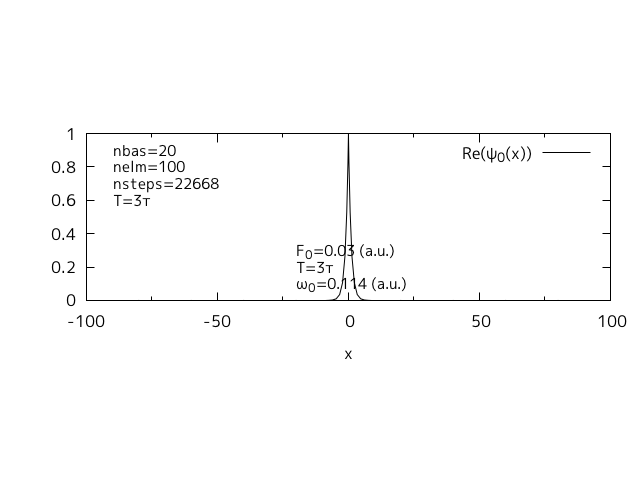
\includegraphics[scale=.20, trim={6 100 0 100},clip]{images/114_f003_3_10_wfc0.png} \\
 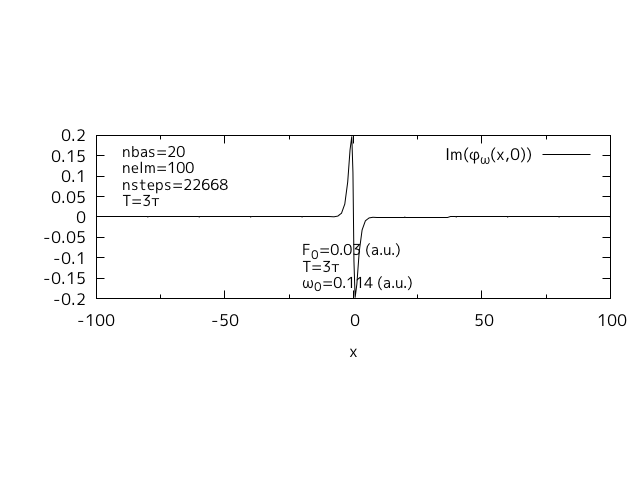
\includegraphics[scale=.20, trim={6 100 0 100},clip]{images/114_f003_3_10_phic0.png} \\
% \includegraphics[scale=.20, trim={6 130 10 100},clip]{images/114_f003_8_03_hhg.png} 
%%\caption{Eigenvalues.}
%\label{fig:pemd_0114}
\end{figure}

\end{minipage}
\end{textblock*}


\begin{textblock*}{500pt}(130pt,60pt)
%\centering
%\rotatebox{90}{
 \begin{minipage}{0.0\linewidth}
 \begin{figure}[tp]
 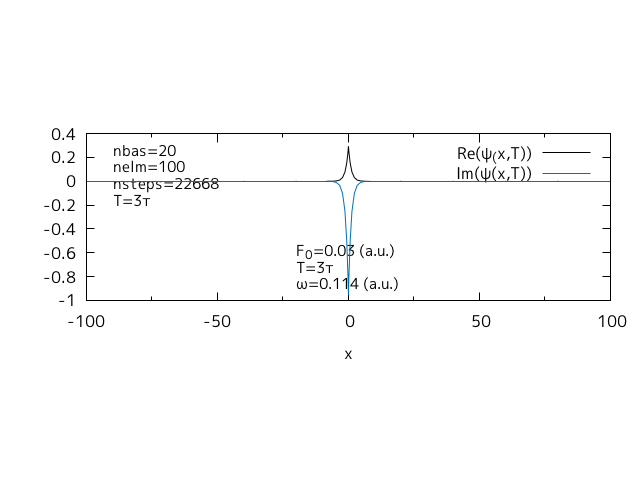
\includegraphics[scale=.20, trim={6 100 0 100},clip]{images/114_f003_3_10_wfc.png} \\
 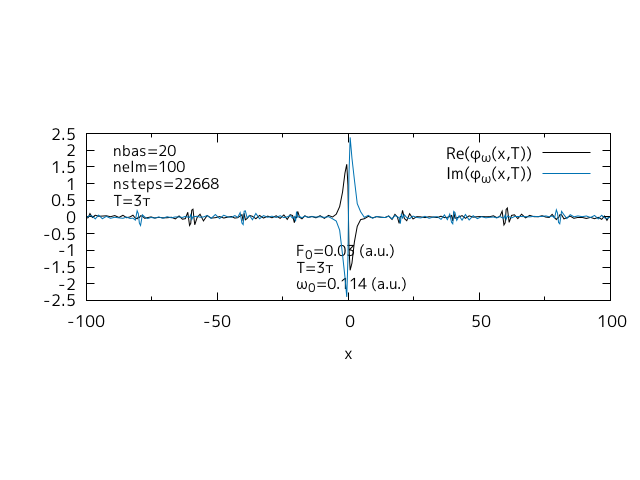
\includegraphics[scale=.20, trim={6 100 0 100},clip]{images/114_f003_3_10_phic.png} \\
% 
\includegraphics[scale=.20, trim={6 130 10 100},clip]{images/114_f003_12_07_hhg.png} 
%%\caption{Eigenvalues.}
%\label{fig:pemd_0114}
 \end{figure}

\end{minipage}
\end{textblock*}


\begin{textblock*}{500pt}(290pt,60pt)
%\centering
%\rotatebox{90}{
 \begin{minipage}{0.0\linewidth}
 \begin{figure}[tp]
 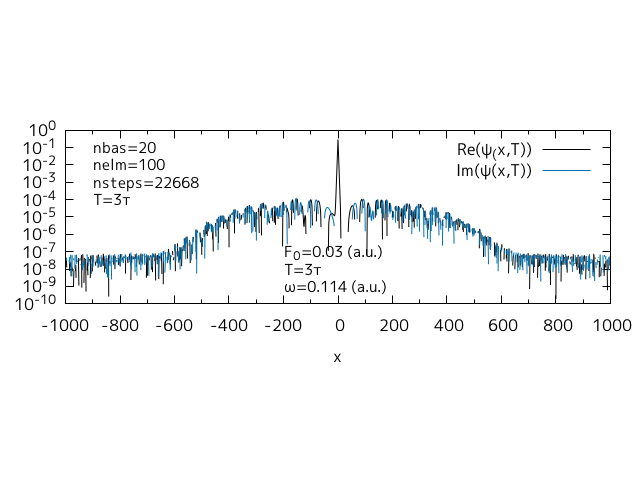
\includegraphics[scale=.20, trim={6 100 0 100},clip]{images/114_f003_3_10_wfc_log.png} \\
 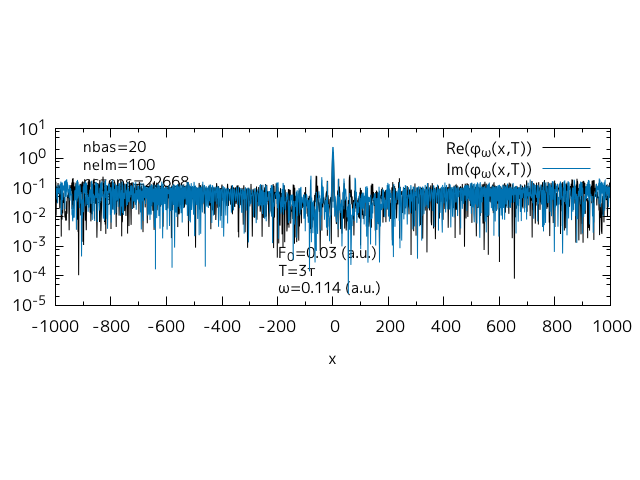
\includegraphics[scale=.20, trim={6 100 0 100},clip]{images/114_f003_3_10_phic_log.png} \\
 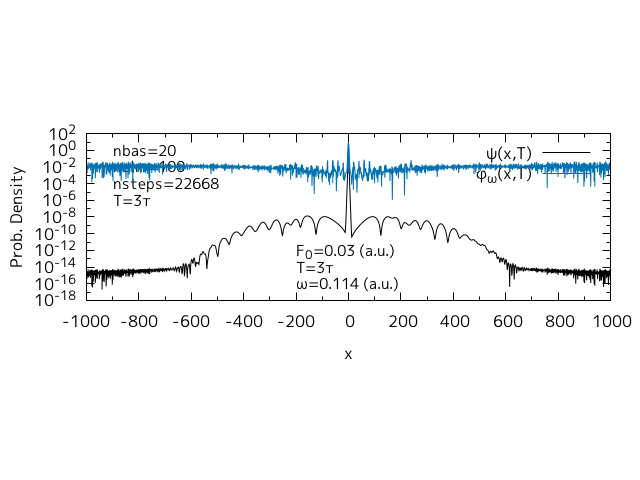
\includegraphics[scale=.20, trim={6 100 0 100},clip]{images/114_f003_3_10_density.png} 
%%\caption{Eigenvalues.}
%\label{fig:pemd_0114}
 \end{figure}

\end{minipage}
\end{textblock*}


\begin{textblock*}{50pt}(30pt,180pt)
\scriptsize
%\begin{itemize}
%\item How to deduce the coefficients of $\phi_\nu$?
\begin{align}
& {\rm nbas}   = 20                 \nonumber\\
& {\rm nelm}   = 100                \nonumber\\ 
& {\rm nsteps} = 22668              \nonumber\\ 
& {\rm xmax}   = 2000               \nonumber\\ 
& T = 3\tau                         \nonumber
\end{align}
%\end{itemize}
\end{textblock*}

\end{frame}





\begin{frame}
\frametitle{Quantum theory of radiation by nonstationary systems 
	with application to high-order harmonic generation
        (Phys. Rev. A 101, 013410 (2020))}
	\framesubtitle{The wavefunction $\phi_\omega(x,t) \;\;\;(\omega=1)$}

\begin{textblock*}{500pt}(5pt,60pt)
%\centering
%\rotatebox{90}{
 \begin{minipage}{0.0\linewidth}
 \begin{figure}[tp]
 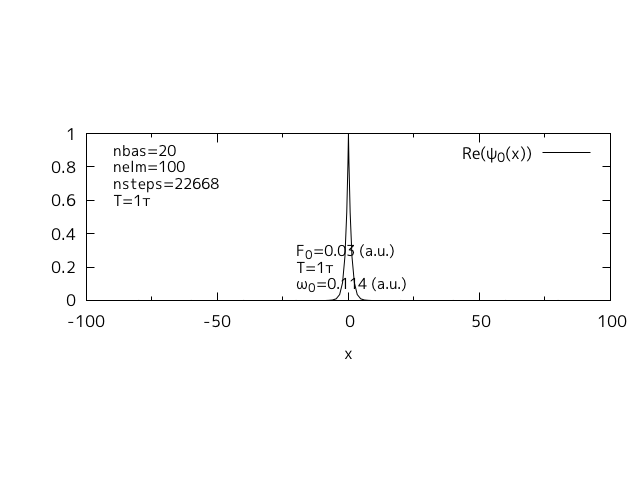
\includegraphics[scale=.20, trim={6 100 0 100},clip]{images/114_f003_1_01_wfc0.png} \\
 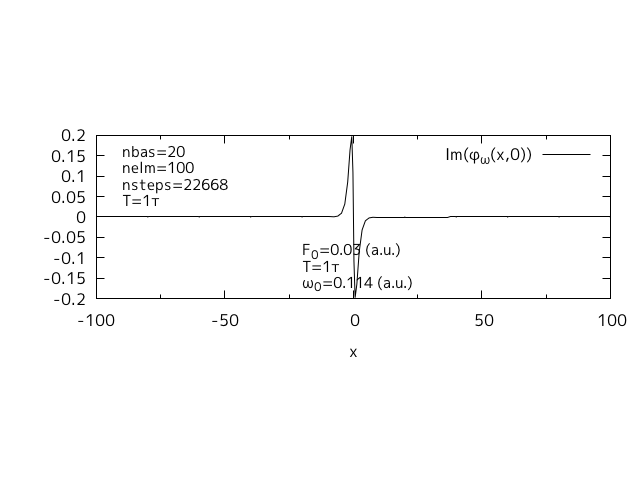
\includegraphics[scale=.20, trim={6 100 0 100},clip]{images/114_f003_1_01_phic0.png} \\
% \includegraphics[scale=.20, trim={6 130 10 100},clip]{images/114_f003_8_03_hhg.png} 
%%\caption{Eigenvalues.}
%\label{fig:pemd_0114}
\end{figure}

\end{minipage}
\end{textblock*}


\begin{textblock*}{500pt}(130pt,60pt)
%\centering
%\rotatebox{90}{
 \begin{minipage}{0.0\linewidth}
 \begin{figure}[tp]
 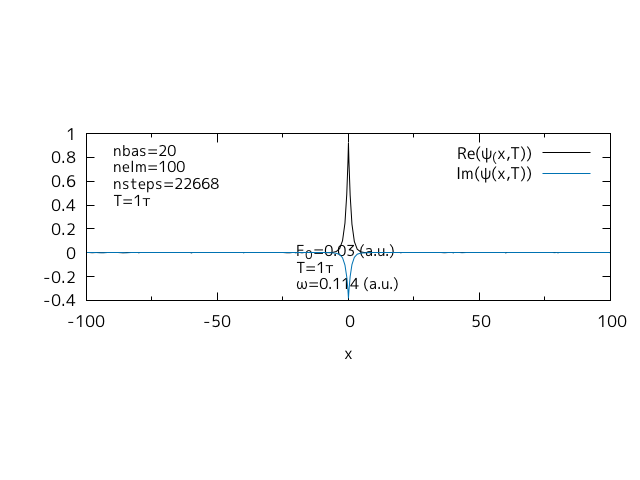
\includegraphics[scale=.20, trim={6 100 0 100},clip]{images/114_f003_1_01_wfc.png} \\
 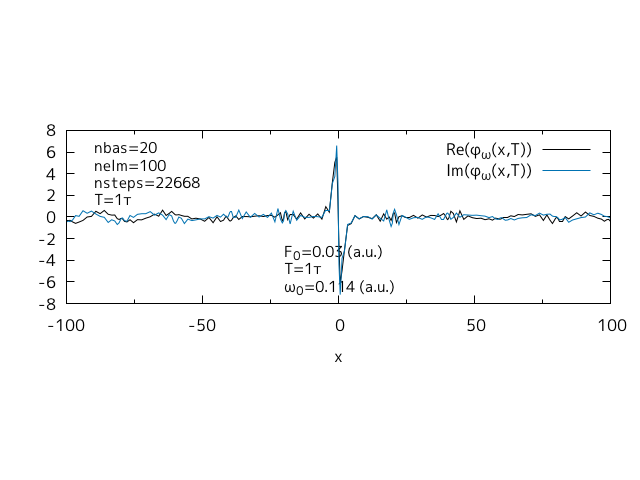
\includegraphics[scale=.20, trim={6 100 0 100},clip]{images/114_f003_1_01_phic.png} \\
% 
\includegraphics[scale=.20, trim={30 130 10 100},clip]{images/114_f003_12_07_hhg.png} 
%%\caption{Eigenvalues.}
%\label{fig:pemd_0114}
 \end{figure}

\end{minipage}
\end{textblock*}


\begin{textblock*}{500pt}(290pt,60pt)
%\centering
%\rotatebox{90}{
 \begin{minipage}{0.0\linewidth}
 \begin{figure}[tp]
 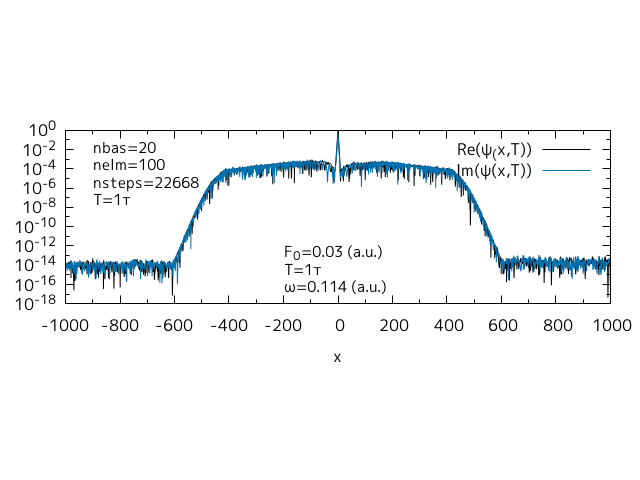
\includegraphics[scale=.20, trim={6 100 0 100},clip]{images/114_f003_1_01_wfc_log.png} \\
 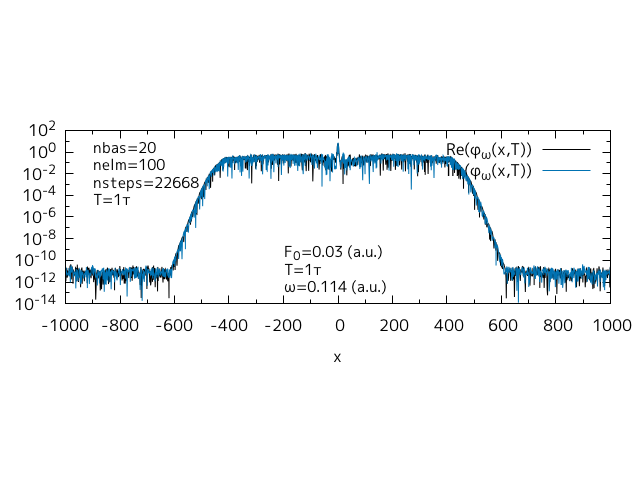
\includegraphics[scale=.20, trim={6 100 0 100},clip]{images/114_f003_1_01_phic_log.png} \\
 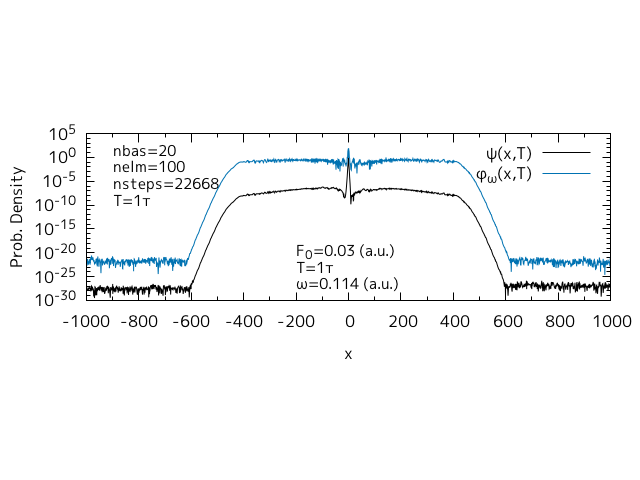
\includegraphics[scale=.20, trim={6 100 0 100},clip]{images/114_f003_1_01_density.png} 
%%\caption{Eigenvalues.}
%\label{fig:pemd_0114}
 \end{figure}

\end{minipage}
\end{textblock*}


\begin{textblock*}{50pt}(30pt,180pt)
\scriptsize
%\begin{itemize}
%\item How to deduce the coefficients of $\phi_\nu$?
\begin{align}
& {\rm nbas}   = 20                 \nonumber\\
& {\rm nelm}   = 100                \nonumber\\ 
& {\rm nsteps} = 22668              \nonumber\\ 
& {\rm xmax}   = 2000               \nonumber\\ 
& T = 1\tau                         \nonumber
\end{align}
%\end{itemize}
\end{textblock*}

\end{frame}





\begin{frame}
\frametitle{Quantum theory of radiation by nonstationary systems 
	with application to high-order harmonic generation
        (Phys. Rev. A 101, 013410 (2020))}
	\framesubtitle{About the field}

\begin{textblock*}{500pt}(5pt,60pt)
%\centering
%\rotatebox{90}{
 \begin{minipage}{0.0\linewidth}
 \begin{figure}[tp]
 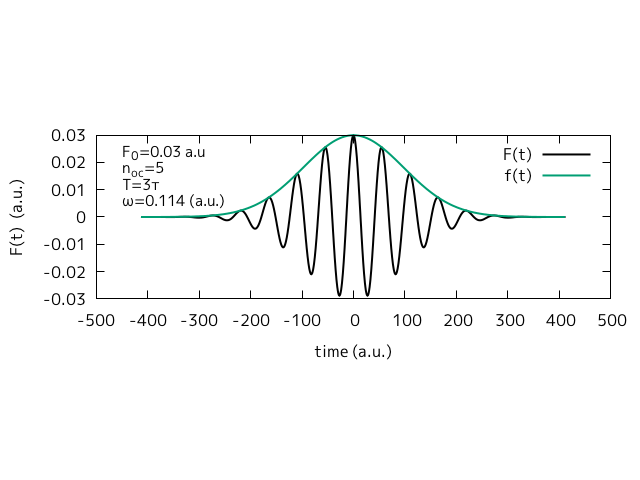
\includegraphics[scale=.20, trim={6 150 10 110},clip]{images/f003_01_114_5_3_field.png} \\
 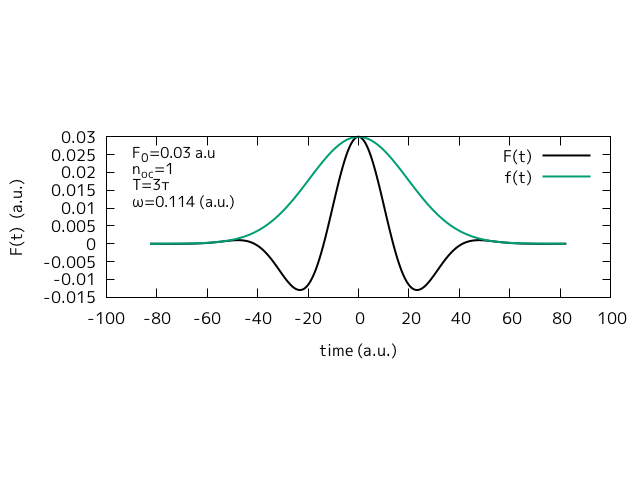
\includegraphics[scale=.20, trim={6 150 10 110},clip]{images/f003_02_114_1_3_field.png} \\
 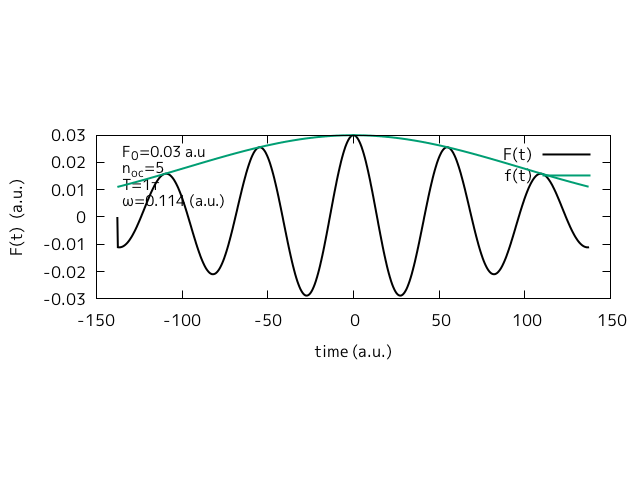
\includegraphics[scale=.20, trim={6 110 10 110},clip]{images/f003_03_114_5_1_field.png} 
%%\caption{Eigenvalues.}
%\label{fig:pemd_0114}
\end{figure}

\end{minipage}
\end{textblock*}


\begin{textblock*}{500pt}(130pt,60pt)
%\centering
%\rotatebox{90}{
 \begin{minipage}{0.0\linewidth}
 \begin{figure}[tp]
 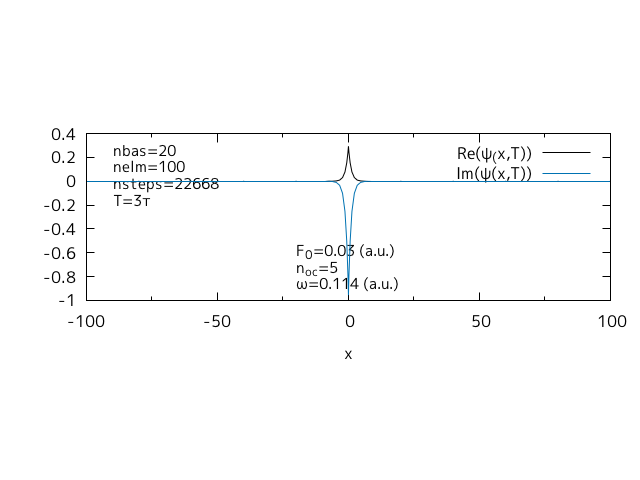
\includegraphics[scale=.20, trim={6 150 10 110},clip]{images/f003_01_114_5_3_wfc.png} \\
 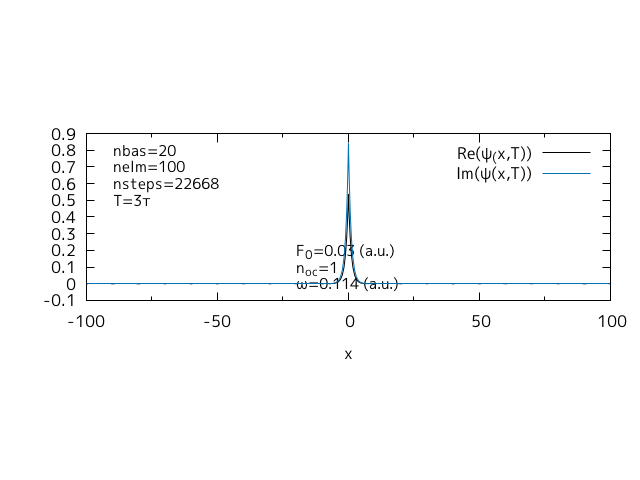
\includegraphics[scale=.20, trim={6 150 10 110},clip]{images/f003_02_114_1_3_wfc.png} \\
 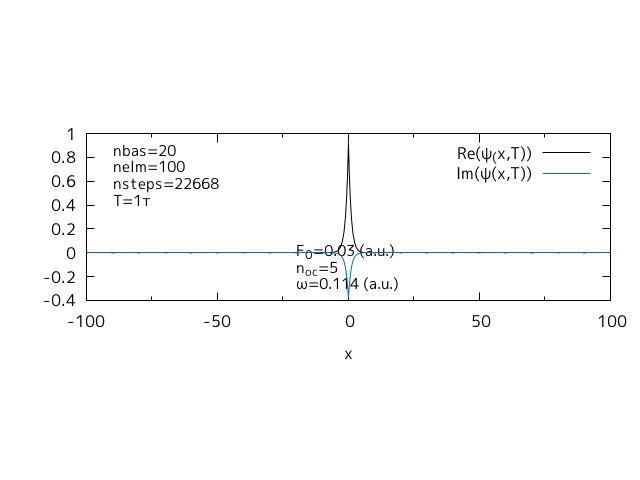
\includegraphics[scale=.20, trim={6 110 10 110},clip]{images/f003_03_114_5_1_wfc.png} 
%%\caption{Eigenvalues.}
%\label{fig:pemd_0114}
 \end{figure}

\end{minipage}
\end{textblock*}


\begin{textblock*}{500pt}(290pt,60pt)
%\centering
%\rotatebox{90}{
 \begin{minipage}{0.0\linewidth}
 \begin{figure}[tp]
 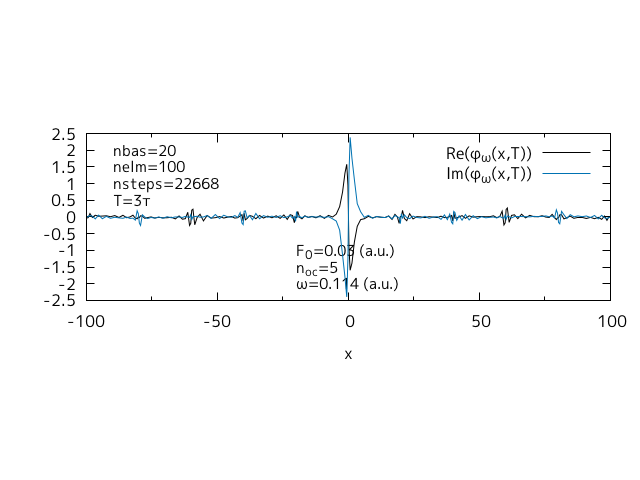
\includegraphics[scale=.20, trim={6 150 10 110},clip]{images/f003_01_114_5_3_phic.png} \\
 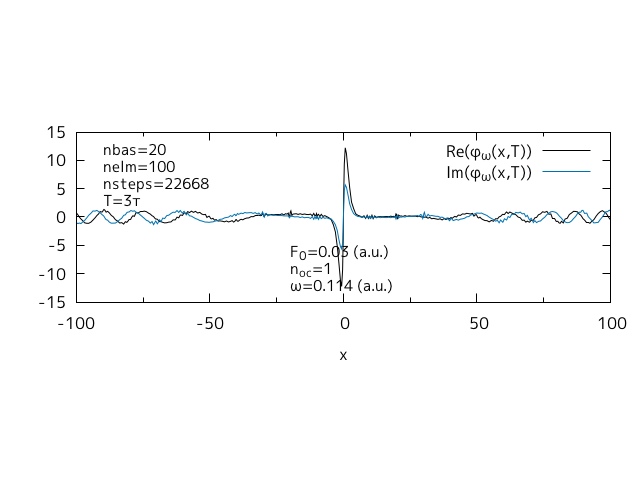
\includegraphics[scale=.20, trim={6 150 10 110},clip]{images/f003_02_114_1_3_phic.png} \\
 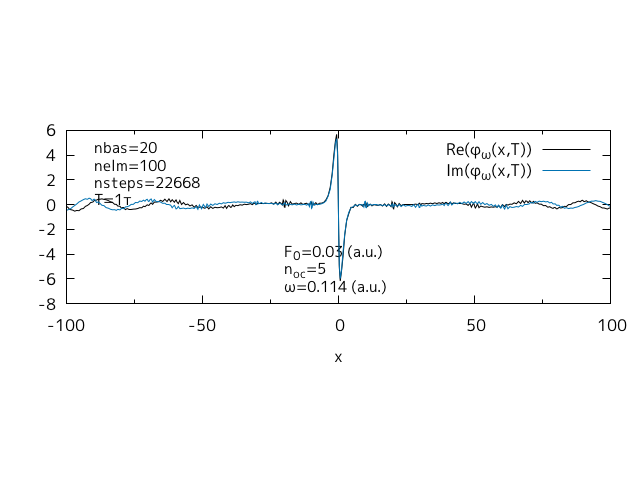
\includegraphics[scale=.20, trim={6 110 10 110},clip]{images/f003_03_114_5_1_phic.png} 
%%\caption{Eigenvalues.}
%\label{fig:pemd_0114}
 \end{figure}

\end{minipage}
\end{textblock*}


%\begin{textblock*}{500pt}(360pt,60pt)
%%\centering
%%\rotatebox{90}{
% \begin{minipage}{0.0\linewidth}
% \begin{figure}[tp]
% 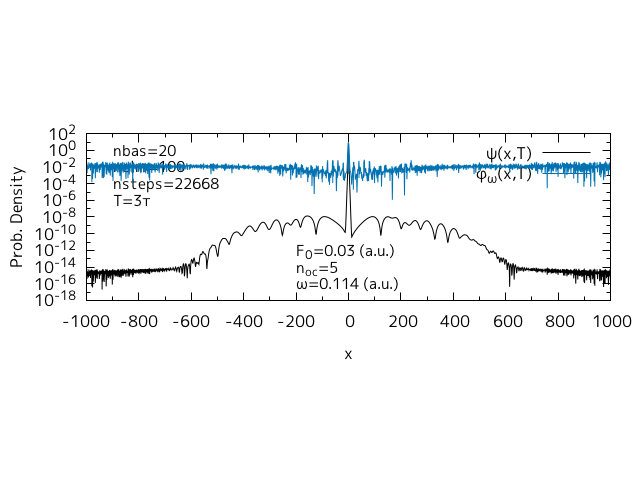
\includegraphics[scale=.20, trim={20 150 10 110},clip]{images/f003_01_114_5_3_density.png} \\
% 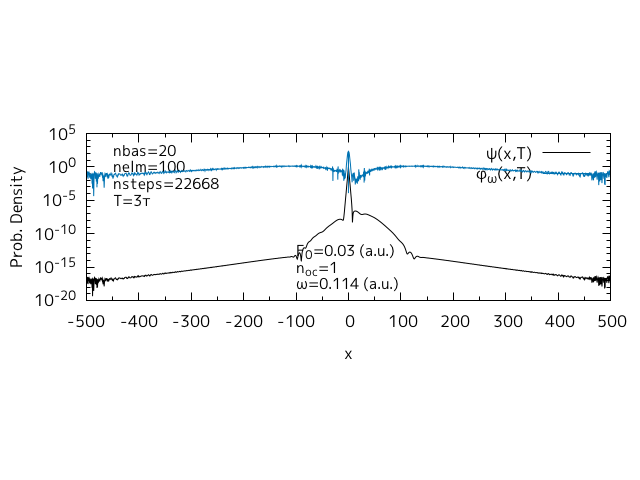
\includegraphics[scale=.20, trim={20 150 10 110},clip]{images/f003_02_114_1_3_density.png} \\
% 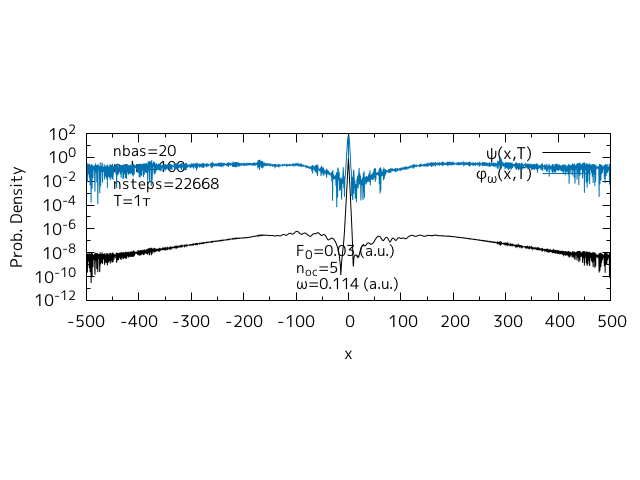
\includegraphics[scale=.20, trim={20 110 10 110},clip]{images/f003_03_114_5_1_density.png} 
%%%\caption{Eigenvalues.}
%%\label{fig:pemd_0114}
% \end{figure}
%
%\end{minipage}
%\end{textblock*}


%\begin{textblock*}{50pt}(30pt,180pt)
%\scriptsize
%%\begin{itemize}
%\begin{align}
%& {\rm nbas}   = 40                 \nonumber\\
%& {\rm nelm}   = 200                \nonumber\\ 
%& {\rm nsteps} = 22668              \nonumber\\ 
%& {\rm xmax}   = 4000               \nonumber\\ 
%& T = 3\tau                         \nonumber
%\end{align}
%%\end{itemize}
%\end{textblock*}

\end{frame}







%\begin{frame}
%\frametitle{Quantum theory of radiation by nonstationary systems 
%	with application to high-order harmonic generation
%        (Phys. Rev. A 101, 013410 (2020))}
%	\framesubtitle{The wavefunction $\phi_\omega(x,t) \;\;\;(\omega=1)$}
%
%\begin{textblock*}{500pt}(5pt,60pt)
%%\centering
%%\rotatebox{90}{
% \begin{minipage}{0.0\linewidth}
% \begin{figure}[tp]
% 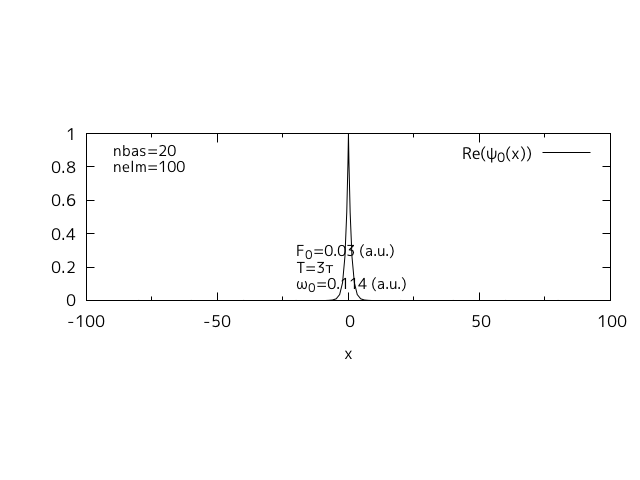
\includegraphics[scale=.20, trim={6 100 0 133},clip]{images/114_f003_3_03_wfc0.png} \\
% 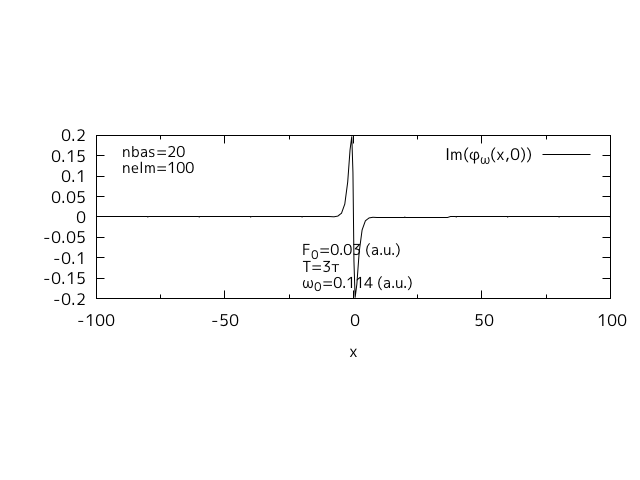
\includegraphics[scale=.20, trim={6 100 0 130},clip]{images/114_f003_3_03_phic0.png} \\
%% \includegraphics[scale=.20, trim={6 130 10 130},clip]{images/114_f003_8_03_hhg.png} 
%%%\caption{Eigenvalues.}
%%\label{fig:pemd_0114}
% \end{figure}
%
%\end{minipage}
%\end{textblock*}
%
%
%\begin{textblock*}{500pt}(130pt,60pt)
%%\centering
%%\rotatebox{90}{
% \begin{minipage}{0.0\linewidth}
% \begin{figure}[tp]
% 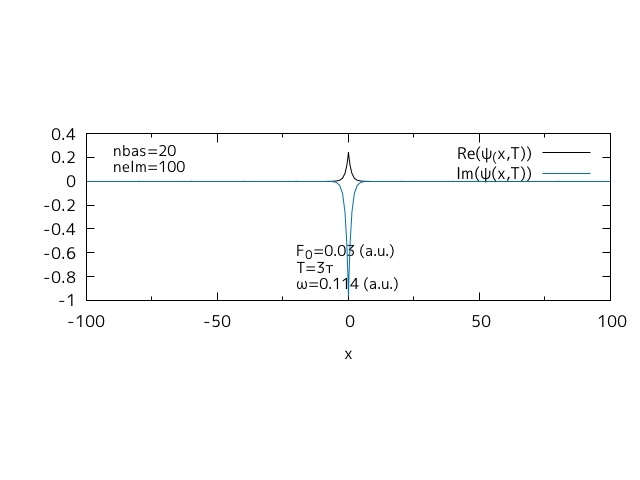
\includegraphics[scale=.20, trim={6 100 0 133},clip]{images/114_f003_3_03_wfc.png} \\
% 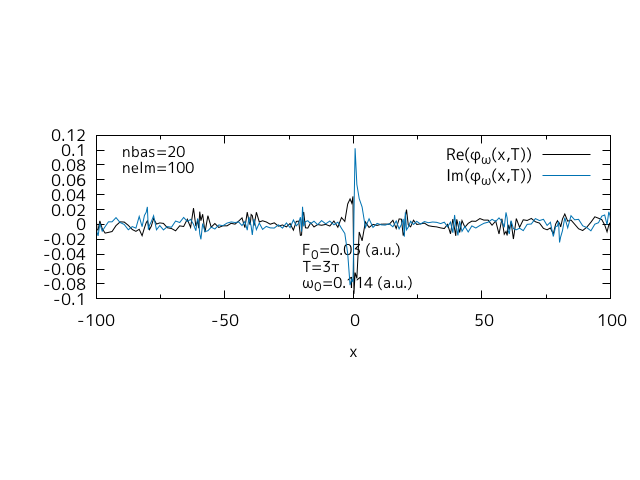
\includegraphics[scale=.20, trim={6 100 0 130},clip]{images/114_f003_3_03_phic.png} \\
%% 
\includegraphics[scale=.20, trim={30 130 10 130},clip]{images/114_f003_12_07_hhg.png} 
%%%\caption{Eigenvalues.}
%%\label{fig:pemd_0114}
% \end{figure}
%
%\end{minipage}
%\end{textblock*}
%
%
%\begin{textblock*}{500pt}(255pt,60pt)
%%\centering
%%\rotatebox{90}{
% \begin{minipage}{0.0\linewidth}
% \begin{figure}[tp]
% 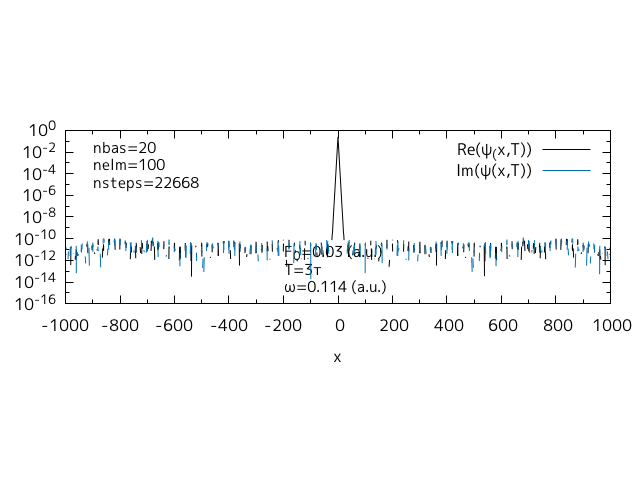
\includegraphics[scale=.20, trim={6 100 0 133},clip]{images/114_f003_3_03_wfc_log.png} \\
% 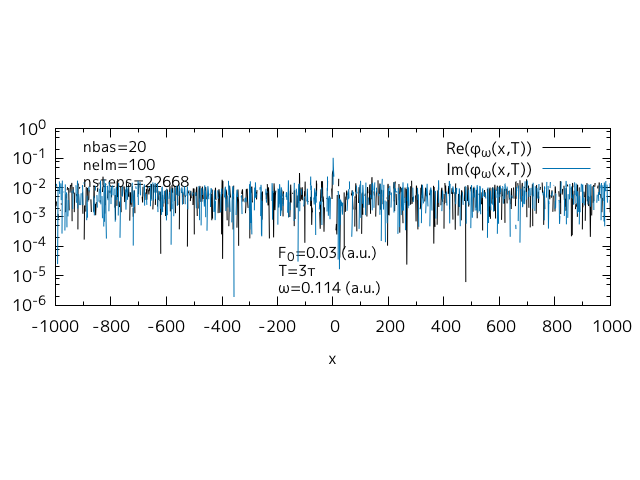
\includegraphics[scale=.20, trim={6 100 0 130},clip]{images/114_f003_3_03_phic_log.png} \\
% 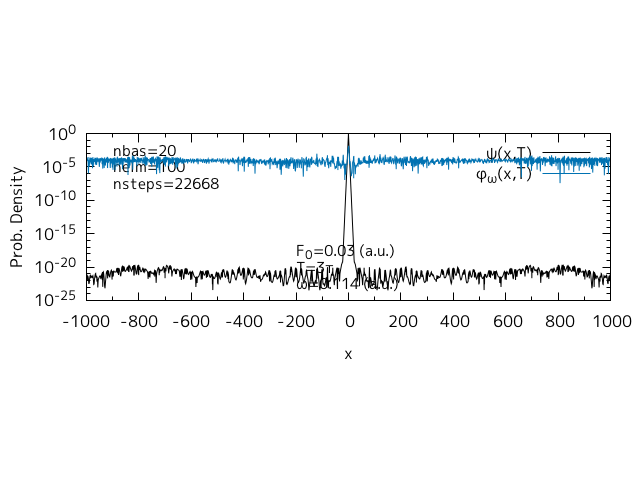
\includegraphics[scale=.20, trim={6 100 0 130},clip]{images/114_f003_3_03_density.png} 
%%%\caption{Eigenvalues.}
%%\label{fig:pemd_0114}
% \end{figure}
%
%\end{minipage}
%\end{textblock*}
%
%
%\begin{textblock*}{400pt}(30pt,200pt)
%\footnotesize
%\begin{itemize}
%\item Laser switched off
%\end{itemize}
%
%\end{textblock*}
%
%
%
%\end{frame}







%\begin{frame}
%\frametitle{Quantum theory of radiation by nonstationary systems 
%	with application to high-order harmonic generation
%        (Phys. Rev. A 101, 013410 (2020))}
%	\framesubtitle{Correct approach}
%
%
%\begin{textblock*}{400pt}(30pt,50pt)
%\footnotesize
%\begin{align}
%  Q_\nu = \alpha^2 \sum_n \left| b_{n\nu}\right|^2 
%\end{align}
%\end{textblock*}
%
%
%\begin{textblock*}{400pt}(30pt,80pt)
%\footnotesize
%\begin{align}
%b_{n\nu}(t\geqslant T) & = b_{n\nu} 
%   + i e^{i(E_n+\omega)t}\langle \psi_n^-|\hat{R}_\nu|\psi(t)\rangle
%\end{align}
%\end{textblock*}
%
%
%
%\begin{textblock*}{400pt}(30pt,100pt)
%\footnotesize
%\begin{align}
%\hat{R}_\nu = \int_0^\infty e^{i\hat{H}_a t}\boldsymbol{A}_\nu
%\hat{\boldsymbol{\rm p}}
%e^{-i\hat{H}_a t} e^{i\omega t - \epsilon t} dt
%\end{align}
%\end{textblock*}
%
%
%\begin{textblock*}{400pt}(30pt,150pt)
%\footnotesize
%\begin{align}
%|\psi(t)\rangle = \sum_n a_n(t) e^{-E_n t}|\psi_n^-\rangle, \\
%|\phi_\nu(t)\rangle = \sum_n b_{n\nu}(t) e^{-E_n t}|\psi_n^-\rangle
%\end{align}
%\end{textblock*}
%
%
%\begin{textblock*}{400pt}(30pt,200pt)
%\footnotesize
%%\begin{itemize}
%%\item How to deduce the coefficients of $\phi_\nu$?
%\begin{align}
%\left.\langle\psi(t)|\phi_\nu(t)\rangle\right|_{t\geqslant T} 
%= \sum_n a_n^*(T) b_{n\nu}(T)
%= -i\boldsymbol{\rm A}_\nu \boldsymbol{\rm p}(\omega), 
%\end{align}
%%\end{itemize}
%\end{textblock*}
%
%
%
%\end{frame}



%\begin{frame}
%\frametitle{Quantum theory of radiation by nonstationary systems 
%	with application to high-order harmonic generation
%        (Phys. Rev. A 101, 013410 (2020))}
%	\framesubtitle{Resolution}
%
%
%\begin{textblock*}{400pt}(30pt,50pt)
%\footnotesize
%\begin{align}
%  Q_\nu = \alpha^2 \sum_n \left| b_{n\nu}\right|^2 
%\end{align}
%\end{textblock*}
%
%
%\begin{textblock*}{400pt}(30pt,80pt)
%\footnotesize
%\begin{align}
%b_{n\nu}(t\geqslant T) & = b_{n\nu} 
%   + i e^{i(E_n+\omega)t}\langle \psi_n^-|\hat{R}_\nu|\psi(t)\rangle
%\end{align}
%\end{textblock*}
%
%
%
%\begin{textblock*}{400pt}(30pt,100pt)
%\footnotesize
%\begin{align}
%\hat{R}_\nu = \int_0^\infty e^{i\hat{H}_a t}\boldsymbol{A}_\nu
%\hat{\boldsymbol{\rm p}}
%e^{-i\hat{H}_a t} e^{i\omega t - \epsilon t} dt
%\end{align}
%\end{textblock*}
%
%
%\begin{textblock*}{400pt}(30pt,150pt)
%\footnotesize
%\begin{align}
%|\psi(t)\rangle = \sum_n a_n(t) e^{-E_n t}|\psi_n^-\rangle, \\
%|\phi_\nu(t)\rangle = \sum_n b_{n\nu}(t) e^{-E_n t}|\psi_n^-\rangle
%\end{align}
%\end{textblock*}
%
%
%\begin{textblock*}{400pt}(30pt,200pt)
%\footnotesize
%%\begin{itemize}
%%\item How to deduce the coefficients of $\phi_\nu$?
%\begin{align}
%\left.\langle\psi(t)|\phi_\nu(t)\rangle\right|_{t\geqslant T} 
%= \sum_n a_n^*(T) b_{n\nu}(T)
%= -i\boldsymbol{\rm A}_\nu \boldsymbol{\rm p}(\omega), 
%\end{align}
%%\end{itemize}
%\end{textblock*}
%
%
%
%\end{frame}
